\documentclass[floatsintext,doc]{apa6}
\usepackage{lmodern}
\usepackage{amssymb,amsmath}
\usepackage{ifxetex,ifluatex}
\usepackage{apacite}
%\usepackage{hyperref}
\usepackage[utf8]{inputenc}
%\usepackage{fourier}%
%\usepackage{fourier}%
%\usepackage{heuristica}
\usepackage{geometry}

\usepackage{array}
\usepackage{tabularx}
\usepackage{caption}

\usepackage{fixltx2e} % provides \textsubscript
\ifnum 0\ifxetex 1\fi\ifluatex 1\fi=0 % if pdftex
  \usepackage[T1]{fontenc}
  \usepackage[utf8]{inputenc}
\else % if luatex or xelatex
  \ifxetex
    \usepackage{mathspec}
  \else
    \usepackage{fontspec}
  \fi
  \defaultfontfeatures{Ligatures=TeX,Scale=MatchLowercase}
\fi
% use upquote if available, for straight quotes in verbatim environments
\IfFileExists{upquote.sty}{\usepackage{upquote}}{}
% use microtype if available
\IfFileExists{microtype.sty}{%
\usepackage{microtype}
\UseMicrotypeSet[protrusion]{basicmath} % disable protrusion for tt fonts
}{}

%\hypersetup{unicode=true,
%            pdftitle={Not unreasonable: Uncertainty in the language of logic},
%            pdfauthor={Michael Henry Tessler~\& Michael Franke},
%            pdfkeywords={semantics; pragmatics; negation; Bayesian cognitive model; Rational Speech Act},
%            pdfborder={0 0 0},
%            breaklinks=true}
%\urlstyle{same}  % don't use monospace font for urls
\usepackage{graphicx,grffile}
\makeatletter
\def\maxwidth{\ifdim\Gin@nat@width>\linewidth\linewidth\else\Gin@nat@width\fi}
\def\maxheight{\ifdim\Gin@nat@height>\textheight\textheight\else\Gin@nat@height\fi}
\makeatother
% Scale images if necessary, so that they will not overflow the page
% margins by default, and it is still possible to overwrite the defaults
% using explicit options in \includegraphics[width, height, ...]{}
\setkeys{Gin}{width=\maxwidth,height=\maxheight,keepaspectratio}
\IfFileExists{parskip.sty}{%
\usepackage{parskip}
}{% else
\setlength{\parindent}{0pt}
\setlength{\parskip}{6pt plus 2pt minus 1pt}
}
\setlength{\emergencystretch}{3em}  % prevent overfull lines
\providecommand{\tightlist}{%
  \setlength{\itemsep}{0pt}\setlength{\parskip}{0pt}}
\setcounter{secnumdepth}{0}
% Redefines (sub)paragraphs to behave more like sections
\ifx\paragraph\undefined\else
\let\oldparagraph\paragraph
\renewcommand{\paragraph}[1]{\oldparagraph{#1}\mbox{}}
\fi
\ifx\subparagraph\undefined\else
\let\oldsubparagraph\subparagraph
\renewcommand{\subparagraph}[1]{\oldsubparagraph{#1}\mbox{}}
\fi

%%% Use protect on footnotes to avoid problems with footnotes in titles
\let\rmarkdownfootnote\footnote%
\def\footnote{\protect\rmarkdownfootnote}



% these packages are needed to insert results 
% obtained from R into the LaTeX document
\usepackage{pgfplotstable}
\usepackage{csvsimple}
\usepackage{siunitx}

% set the name of the folder in which the CSV files with 
% information from R is stored
\newcommand{\datafoldername}{csv_data_4_tex}

% the following code defines the convenience functions
% as described in the main text below

% rlgetvalue returns whatever is the in cell of the CSV file
% be it string or number; it does not format anything
\newcommand{\rlgetvalue}[4]{\csvreader[filter strcmp={\mykey}{#3},
             late after line = {{,}\ }, late after last line = {{}}]
            {\datafoldername/#1}{#2=\mykey,#4=\myvalue}{\myvalue}}

% rlgetvariable is a shortcut for a specific CSV file (myvars.csv) in which
% individual variables that do not belong to a larger chunk can be stored
\newcommand{\rlgetvariable}[1]{\csvreader[]{\datafoldername/myvars.csv}{#1=\myvar}{\myvar}\xspace}

% rlnum format a decimal number
\newcommand{\rlnum}[2]{\num[output-decimal-marker={.},
                             exponent-product = \cdot,
                             round-mode=places,
                             round-precision=#2,
                             group-digits=false]{#1}}

\newcommand{\rlnumsci}[2]{\num[output-decimal-marker={.},
                          scientific-notation = true,
                             exponent-product = \cdot,
                             round-mode=places,
                             round-precision=#2,
                             group-digits=false]{#1}}

\newcommand{\rlgetnum}[5]{\csvreader[filter strcmp={\mykey}{#3},
             late after line = {{,}\ }, late after last line = {{}}]
            {\datafoldername/#1}{#2=\mykey,#4=\myvalue}{\rlnum{\myvalue}{#5}}}

\newcommand{\rlgetnumsci}[5]{\csvreader[filter strcmp={\mykey}{#3},
             late after line = {{,}\ }, late after last line = {{}}]
            {\datafoldername/#1}{#2=\mykey,#4=\myvalue}{\rlnumsci{\myvalue}{#5}}}

\newcommand{\brmresults}[2]{\(\beta = \rlgetnum{#1}{key}{#2}{mean}{3}\) (\rlgetnum{#1}{key}{#2}{l95}{3}, \rlgetnum{#1}{key}{#2}{u95}{3})}
\newcommand{\brmresultsp}[2]{\(\beta = \rlgetnum{#1}{key}{#2}{mean}{3}\) [\rlgetnum{#1}{key}{#2}{l95}{3}, \rlgetnum{#1}{key}{#2}{u95}{3}]}
\newcommand{\effsize}[2]{\(d = \rlgetnum{#1}{key}{#2}{mean}{2}\) [\rlgetnum{#1}{key}{#2}{l95}{2}, \rlgetnum{#1}{key}{#2}{u95}{2}]}




%  \title{Not unreasonable: Uncertainty in the language of negation}
%  \title{Not unreasonable: Multiple opposite meanings are entertained when understanding negation}
%\title{Not stating the opposite: Negation as an uncertain operation}
%\title{Two negatives don't exactly make a positive}
\title{Not unreasonable: Why two negatives don't make a positive}
    \author{Michael Henry Tessler\textsuperscript{1,3}~\& Michael Franke\textsuperscript{2}}
    \date{}
  
\shorttitle{Flexible negation in language}
\affiliation{
\vspace{0.5cm}
\textsuperscript{1} Massachusetts Institute of Technology, Department of Brain and Cognitive Sciences\\\textsuperscript{2} University of Osnabr\"{u}ck, Department of Cognitive Sciences\\\textsuperscript{3} Stanford University, Department of Psychology}
\keywords{language; pragmatics; negation; Bayesian cognitive model; Rational Speech Act  \newline\indent Word count: 4129}
\usepackage{csquotes}
\usepackage{upgreek}
\captionsetup{font=singlespacing,justification=justified}

\usepackage{longtable}
\usepackage{lscape}
\usepackage{multirow}
\usepackage{tabularx}
\usepackage[flushleft]{threeparttable}
\usepackage{threeparttablex}

%\newenvironment{lltable}{\begin{landscape}\begin{center}\begin{ThreePartTable}}{\end{ThreePartTable}\end{center}\end{landscape}}

\makeatletter
\newcommand\LastLTentrywidth{1em}
\newlength\longtablewidth
\setlength{\longtablewidth}{1in}
\newcommand{\getlongtablewidth}{\begingroup \ifcsname LT@\roman{LT@tables}\endcsname \global\longtablewidth=0pt \renewcommand{\LT@entry}[2]{\global\advance\longtablewidth by ##2\relax\gdef\LastLTentrywidth{##2}}\@nameuse{LT@\roman{LT@tables}} \fi \endgroup}


%\DeclareDelayedFloatFlavor{ThreePartTable}{table}
%\DeclareDelayedFloatFlavor{lltable}{table}
%\DeclareDelayedFloatFlavor*{longtable}{table}
\makeatletter
%\renewcommand{\efloat@iwrite}[1]{\immediate\expandafter\protected@write\csname efloat@post#1\endcsname{}}
\makeatother
\usepackage{tabularx}
\usepackage{multicol}
\usepackage{wrapfig}
\usepackage{gensymb}
\usepackage{tikz}
\usepackage{caption}
\usepackage{booktabs}
\usepackage{xcolor}

\usepackage{xspace}
\newcommand{\ourmodel}{Flexible Negation\xspace}


\authornote{This work was supported in part by NSF Graduate Research Fellowship DGE-114747 to MHT.

Correspondence concerning this article should be addressed to Michael Henry Tessler, 43 Vassar St, Cambridge, MA 02139. E-mail: \url{tessler@mit.edu}}

%\abstract{
%Logic tells us that two negatives make a positive, but in natural language, things are not so black and white: A person \emph{not unhappy} may not be entirely \emph{happy}.
%We hypothesize that innovative uses of double negatives like \emph{not unhappy} stem from listeners entertaining multiple meanings for negation markers like \emph{not} and \emph{un-}, which context can then help disambiguate. 
% %; then, a speaker who uses two negations signals that she intends the negations in a nonredundant manner.
%%We often want to express the exact opposite of a proposition, but natural languages provide multiple ways of stating the opposite: A person who is \emph{not happy} might be \emph{unhappy}, \emph{sad}, or perhaps neither, just \emph{not happy}. Intuition suggests, contra standard logic, that two negatives do not make a positive but rather create nonredundant meanings: 
%%Rather than being redundant, we hypothesize that negation markers entertain a multiplicity of possible meanings, which allows allows listeners to derive fine-grained distinctions among semantically equivalent alternatives. 
%%We formalize this hypothesis in a computational model of language understanding and show that double negations are predicted to have more subtle meanings than their associated simple positive expressions (like \emph{happy}).
%We formalize this hypothesis in a computational model of language understanding, which predicts that \emph{not unhappy} means something different than simple \emph{happy} but also makes surprising additional predictions about single negations (\emph{unhappy}~vs.~\emph{not happy}): The two mean the same thing when presented in isolation, but not when a speaker uses both in the same context. %, \emph{unhappy} should be more negative than \emph{not happy}. 
%The most radical view of uncertainty in negation additionally predicts that an utterance involving the same negation marker twice (e.g., \emph{not not happy}) should mean something different than just \emph{happy}.
%Three experiments confirm consistent orderings of interpretations that interact with the presentational context in the way predicted.
%These findings suggest that even one of the most logical elements of language---negation---can mean many things at once.}

\abstract{
Logic tells us that two negatives make a positive, but in language, things are not so black and white: A person \emph{not unhappy} may not be entirely \emph{happy}. We hypothesize that non-logical uses of double negatives like \emph{not unhappy} stem from listeners entertaining flexible meanings for negation markers like \emph{not} and \emph{un-}, which context can then help disambiguate. We formalize this hypothesis in a computational model of language understanding, which predicts that \emph{not unhappy} means something different than \emph{happy} while also entertaining that single negations (\emph{unhappy} and \emph{not happy}) can be interpreted identically when context does not suggest otherwise. 
Across three experiments ($n= 995$), we confirm these predictions experimentally and further find that double negations that flagrantly use the same negation marker twice (e.g., \emph{not not happy}) can also be interpreted in subtle ways.  
These findings argue against simplistic assumptions of language---even logical elements in language---often used throughout psychological science.
}

\begin{document}
\maketitle

\newcommand*\diff{\mathop{}\!\mathrm{d}}
\newcommand{\denote}[1]{\mbox{ $[\![ #1 ]\!]$}}
\newcommand{\tableref}[1]{Table$\thinspace$\ref{#1}}
\newcommand{\figref}[1]{Fig.$\thinspace$\ref{#1}}
\newcommand{\appref}[1]{Appendix \ref{#1}}
\newcommand{\sectionref}[1]{Section \ref{#1}}
\definecolor{Red}{RGB}{255,0,0}
\definecolor{Green}{RGB}{10,200,100}
\definecolor{Blue}{RGB}{10,100,200}
\definecolor{grey}{RGB}{40,40,40}

\newcommand{\red}[1]{\textcolor{Red}{#1}}  
\newcommand{\mf}[1]{\textcolor{Green}{[mf: #1]}}  
\newcommand{\mht}[1]{\textcolor{Blue}{[mht: #1]}}

%\newcommand{\wrapmf}[1]{#1}

\providecommand{\tightlist}{%
  \setlength{\itemsep}{0pt}\setlength{\parskip}{0pt}}
\newpage


%\begin{quote}
%\emph{When Mr. Collins said any thing of which his wife might reasonably be ashamed, which certainly was not unseldom, she involuntarily turned her eye on Charlotte.}
%(Pride and Prejudice) \mf{Is  this example ideal? It reads to me like a ``damn well often'' case mentioned at the very end of the paper as well.}
%\end{quote}

%\begin{quote}
%\emph{Although Buck wished he could live with his family, his journal entries paint a picture of a man who was a little bored but not unhappy.}
%\cite{marten2011sing} (p.197) 
%\end{quote}

%\begin{quote}
%\emph{The silence of history seems to prove this much, that Sheshian was not unhappy under their unrenowned administration; and to be not unhappy, is at least a very tolerable condition.}
%(Belle Assemblée: Or, Court and Fashionable Magazine; Containing Interesting and Original Literature, and Records of the Beau-monde, Volume 1, Part 2)
%\end{quote}
%
%\begin{quote}
%\emph{I've been waiting for you all week. Don't you know that it is a rotten time to not not be me?}
%(El-P, ``Works every time (feat.~Paul Banks)'') 
%\end{quote}

\begin{quote}\emph{Banal statements are given an appearance of profundity by means of the ``not un-'' formation. [$\ldots$] It should be possible to laugh the ``not un-'' formation out of existence by memorizing this sentence: ``A not unblack dog was chasing a not unsmall rabbit across a not ungreen field.'' }
\cite{orwell1946politics} (p.$\thinspace$357)
%(Orwell, 1946; )
\end{quote}


%\hypertarget{introduction}

Language conveys our thoughts, but we think and feel in ways that are challenging to express in words.
Occasionally, speakers will coin a new term to express a subtle feeling, like being ``plateaued'' \cite{bardwick1986plateauing} or residing in a ``zone of indifference'' \cite{sapir1944grading}.
But we also use the linguistic devices already available to us to create new, perhaps delicate meanings (e.g., through metaphors; \citeNP{lakoff2008}).
 %to navigate and communicate the gradations of our thoughts and feelings 
 
The creation of novel meanings from familiar parts is on ready display in constructions involving two negations: A person \emph{not unhappy} is probably not entirely happy.
The interpretation of double negatives is important from a logical perspective \cite{Horn1989:Natural, Krifka2007:Negated-antonyms} as well as a legal one, where such constructions are surprisingly common \cite{tiersma1999legal}.
%Also,
% insofar as novel meanings can be expressed through the iterative application of the same logical operation (i.e., two negatives), 
Understanding why somebody would say a double negative like \emph{I'm not unhappy} could also provide a window into richer conceptual spaces like emotions \cite{Lindquist2015, Satpute2016}, where the usage of negation can modulate physiological responses \cite{Herbert2011}.
More broadly, pinning down the meaning of such a logical element of language as negation is crucial for so much of psychological science that depends upon using linguistic information to convey task instructions and content.

%Metaphoric language is an obvious example \cite<e.g.,>{lakoff2008}
% \red{(something from the reference game using impoverished language / language evolution / convention formation literature?)}. 


%\emph{how does it feel to be not unhappy}?;

%Compositionality enables productive language use, and double negations are a classic example of using simple linguistic tools to convey subtle meanings.
%One can easily express the opposite of a feeling by deploying a negation marker, but sometimes multiple options exist. 
%One could say ``I'm not happy'' or ``I'm unhappy''. 
%In logic, two negatives make a poitive, but in natural language, that does not seem to be the case:
%When Obama said that the time to negotiate was \emph{not unlimited}, why did he not just say that the time was limited? 
%If Mary is \emph{not unhappy}, does that mean she is \emph{happy}?
%It doesn't seem exactly right:

%\citeA{Jespersen1924} suggested not:

A common, intuition about the meaning of double negatives is expressed by \citeA{Jespersen1924}:
\begin{quote}
[T]wo negatives do not exactly cancel one another [$\ldots$]; the longer expression is always weaker: ``this is not unknown to me''  [$\ldots$] means ``I am to some extent aware of it,'' etc. \cite{Jespersen1924} (p.$\thinspace$332) 
\end{quote}
\noindent In other words, \emph{not unhappy} (a \emph{negated antonym}) should indicate a slightly positive state, below that of \emph{happy}  but perhaps more positive than neutral (i.e., above the zone of indifference; \citeNP{sapir1944grading}). %, where feelings that are neither positive nor negative reside. 
These intuitions are subtle, not universally agreed upon, and further complicated by the fact that the meaning of double negations (\emph{not unhappy})  invariably depends upon the meaning of the component, single negations (\emph{not happy}, \emph{unhappy}), which are also difficult to pin down. % are also not obviously different from one another.
Some argue the single negations have the same meaning \cite<e.g., \emph{not happy} = \emph{unhappy};>{Jespersen1917:Negation, Blutner2004:pragmatics}, while others disagree \cite<e.g.,>{Krifka2007:Negated-antonyms}, citing examples like:


%Standard approaches to understanding the meaning of linguistic expressions in context often involve reasoning about what not only what a speaker said but what else a speaker could have said \cite{Grice1975}.
%For example,


\begin{quote}
It's an absolutely horrible feeling to be unhappy, and I don't even think I was unhappy, just not happy, if you know what I mean.%\emph{(taken from the internet)}
\end{quote}



\begin{figure}[t]
\center 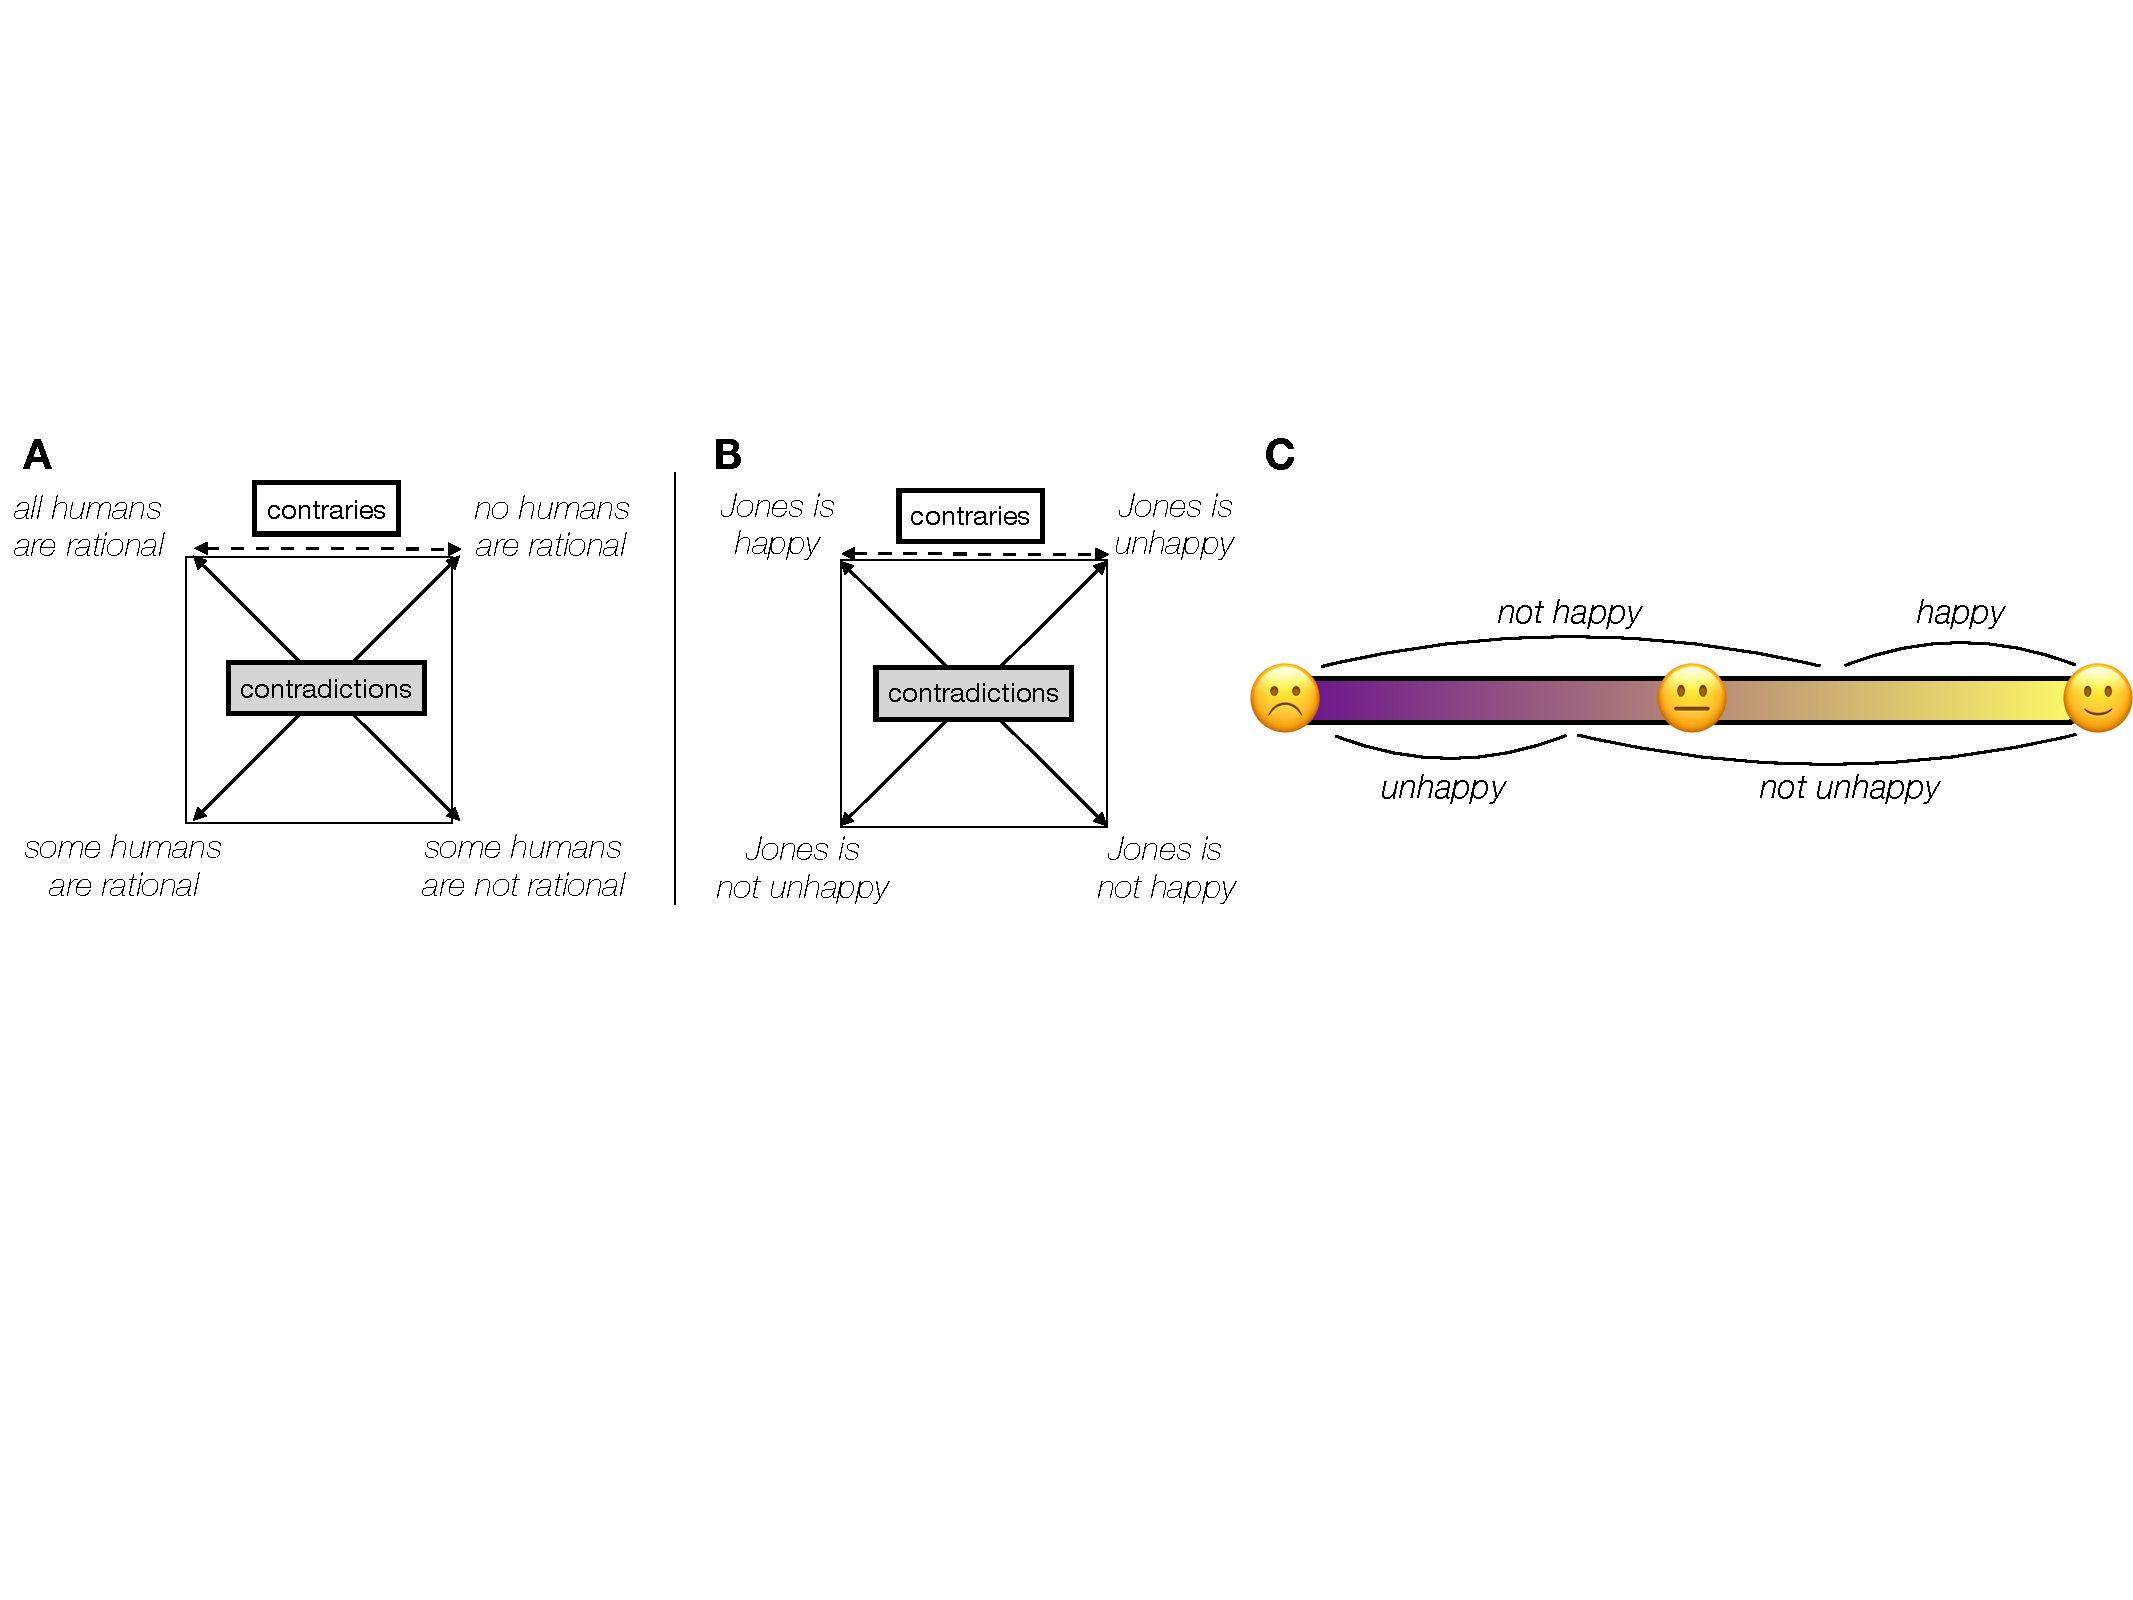
\includegraphics[width=1\textwidth]{figs/opp-square2}  
\caption{Contraries and contradictions as two different kinds of negation. A: Aristotle's classic square of opposition applied to quantifiers (all, some, none). B: An Aristotelean analysis of negated antonyms (happy, unhappy, not unhappy). C: Interpretations of negated antonyms in terms of \emph{degrees of happiness} under an Aristotelean analysis.}\label{fig:opp-square}
\end{figure}


Theorizing about the meaning of negation goes back to Aristotle, who noted that there are multiple ways of conveying an opposite meaning.
\emph{Contradictory} opposites must have opposite truth values, e.g., \enquote{No humans are rational} and \enquote{Some humans are rational}. 
\emph{Contrary} opposites cannot both be true, but can both be false, e.g., \enquote{All humans are rational} and \enquote{No humans are rational}  (Figure \ref{fig:opp-square}A). 
Thus, a straightforward Aristotelean hypothesis would assign one negation marker (\emph{not}) to be a contradictory opposite and another (\emph{un-}) to be a contrary (Figure \ref{fig:opp-square}B); a double negative (\emph{not unhappy}) in this analysis would convey a contradiction of a contrary, resulting in a meaning distinct from that of the positive adjective (\emph{happy}), while also enforcing a difference between the two single negations (\emph{unhappy} $<$ \emph{not happy}) (Figure \ref{fig:opp-square}C; \citeNP{Horn1989:Natural, Horn1991:Duplex, Krifka2007:Negated-antonyms}).
An Orwellian analysis (\emph{a la} the quote in the Preamble), on the other hand, only acknowledges contradictory opposition (\emph{unhappy} $=$ \emph{not happy}) and two negatives would be entirely redundant \cite<\emph{not unhappy} = \emph{happy}; Figure \ref{fig:happy-scale};>{orwell1946politics}.\footnote{Models are named mnemonically. Aristotle and Orwell did not defend these models themselves.}
Perhaps neither Aristotle nor Orwell got it exactly right: the logical distinction between contradictory~vs.~contrary opposition could create an ambiguity in the meanings of negation markers such that either ``not'' or ``un-'' could be used to form either a contrary or contradiction \cite<e.g.,>{russell1905denoting, martin1982negation, wessel1993}, and listeners must represent and reason over this uncertainty when interpreting negations in language (Figure \ref{fig:meanings}).
We develop this hybrid alternative as a \ourmodel hypothesis.

% Formally, a contradictory opposition turns a predicate $H$ into $\neg H$, and contradictory opposition can be iterated ($\neg \neg H$; e.g., \emph{the enemy of my enemy is my friend}).
% Contrary opposition turns $H$ into a new predicate $\tilde{H}$, but standard logic does not allow for the iteration of contrary opposition (i.e., $\tilde{\tilde{H}}$ is not a logical possibility;  \citeNP{Horn1989:Natural}).


%How should negations that use the particle \emph{not} and those formed by morphology (\emph{un-}, \emph{in-}, \emph{im-}, \emph{dis-}, etc.) map onto contraries~vs.~contradictions?

% \footnote{Though we refer to these models as \emph{Aristotle} and \emph{George Orwell}, they are derived from different mappings of English negation markers onto logical operations. Aristotle did not speak English, and thus would personally have not had much to say about \emph{not} or \emph{un-} as we understand them. George Orwell was an English speaker, though not a formal linguist or scientist. The important feature of these individuals was that their ideas have natural analogues to the semantic question we ask here.}

\begin{figure}[t]
\centering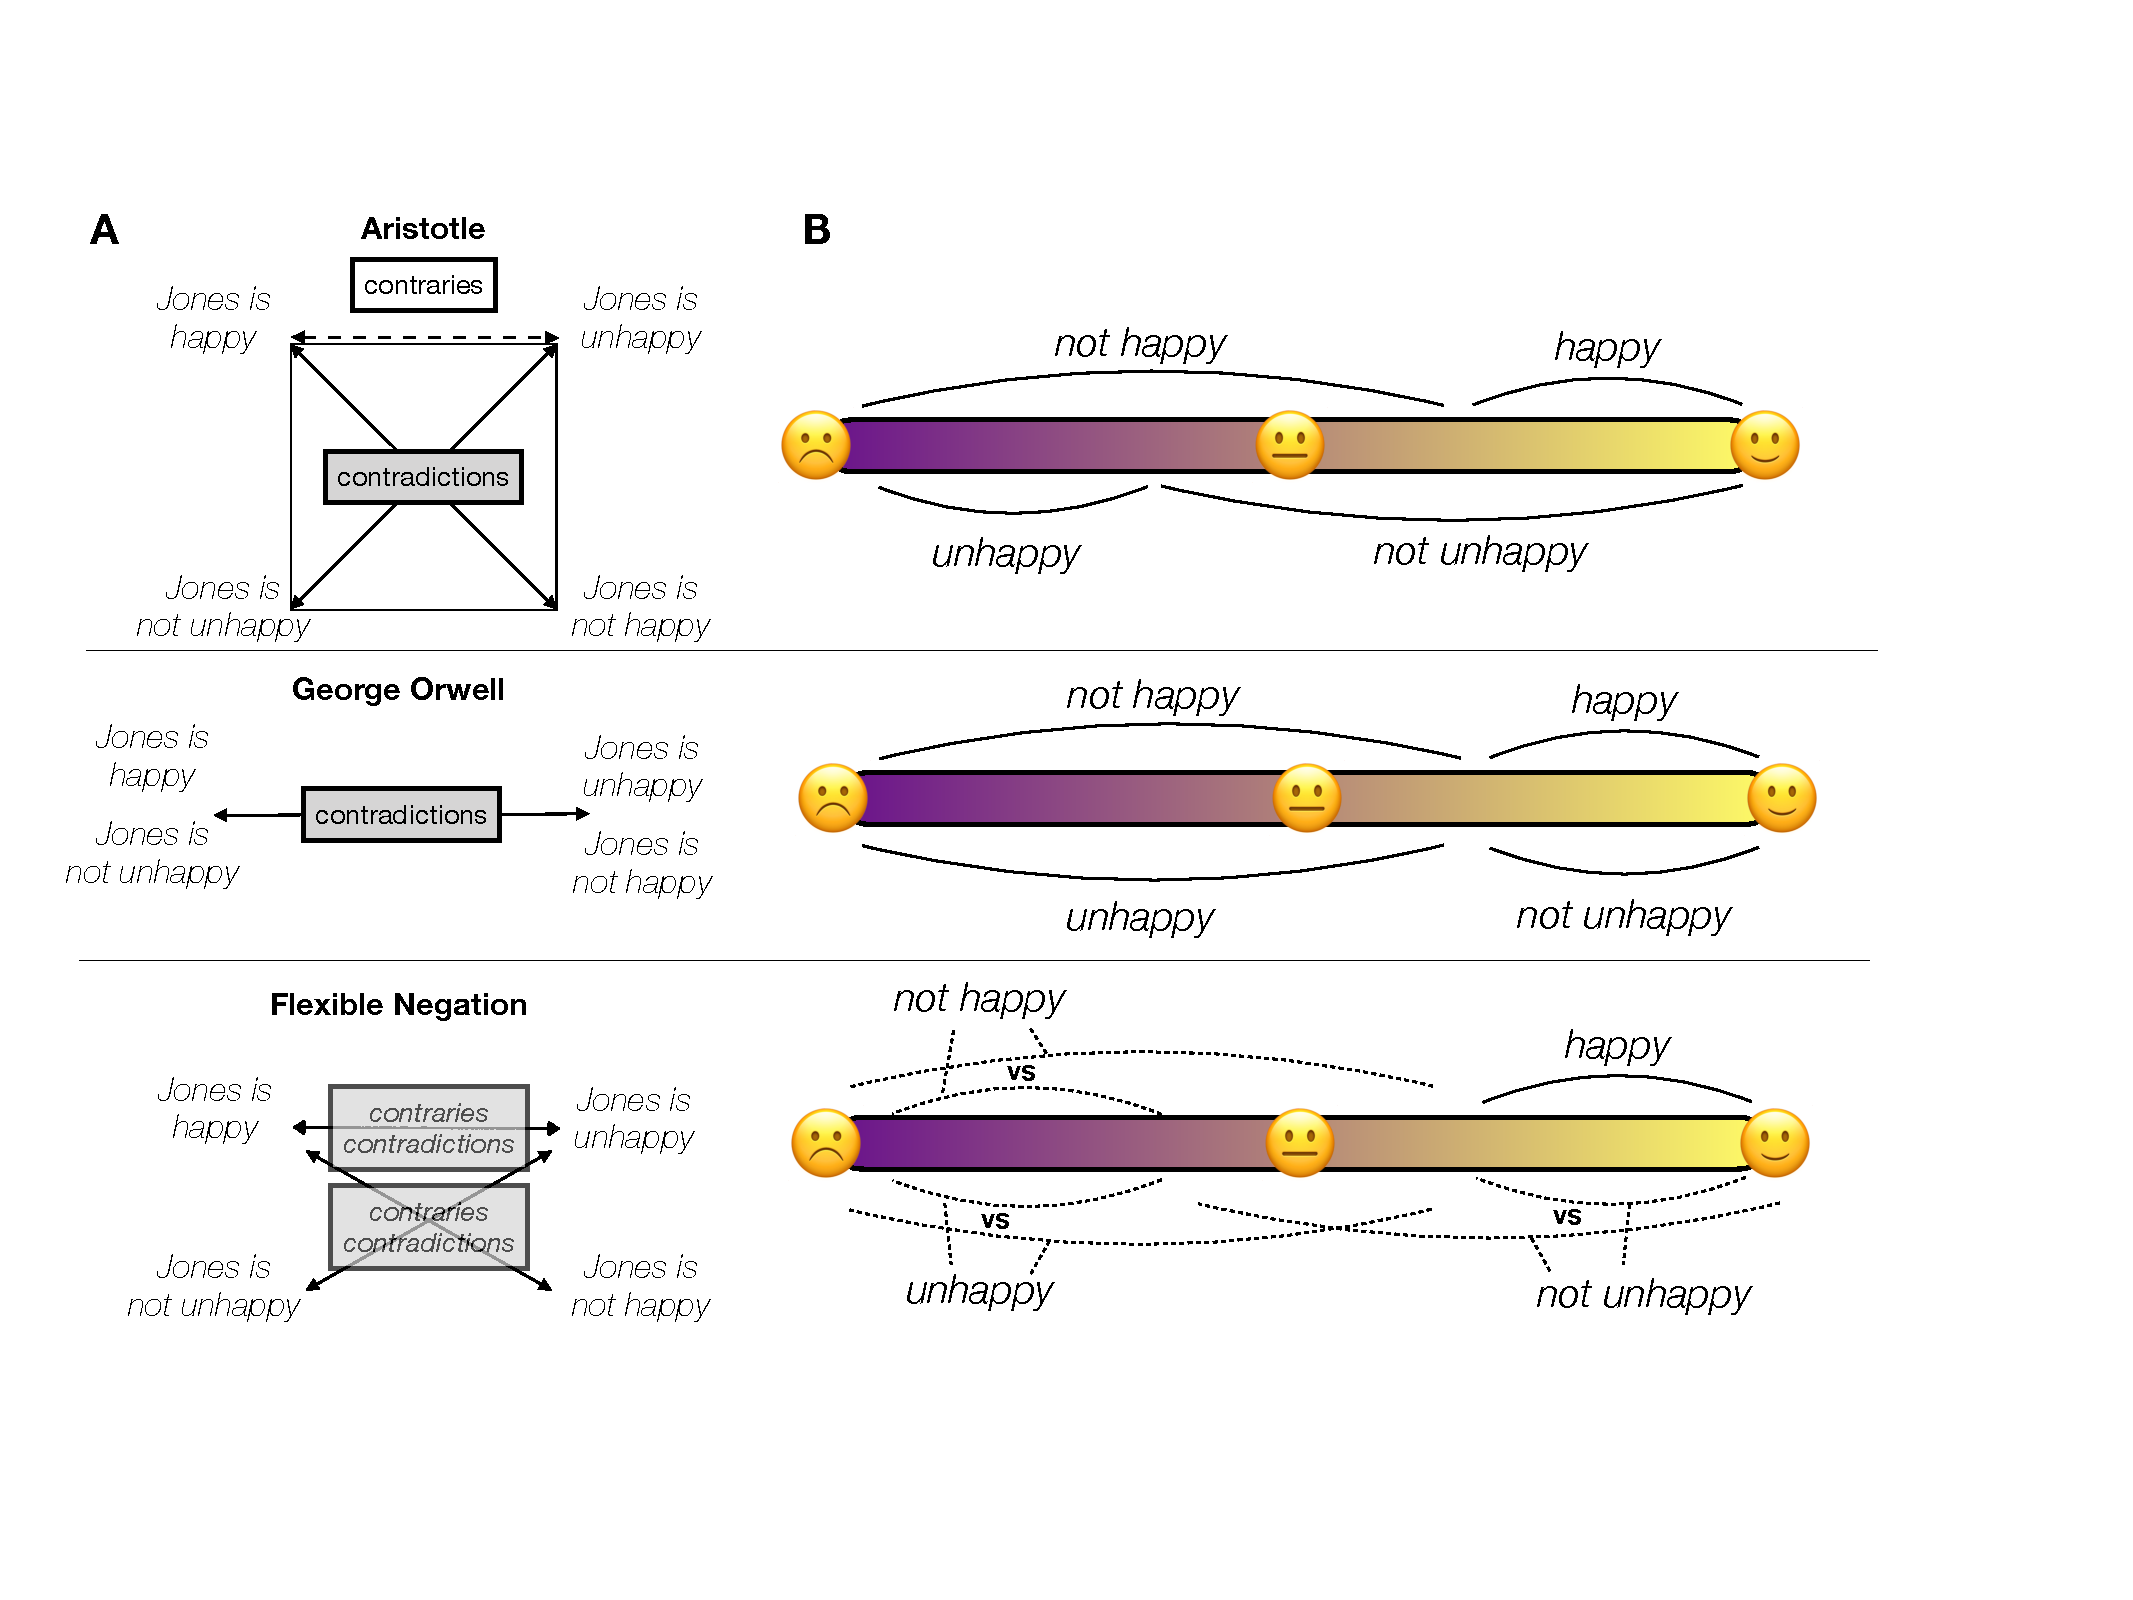
\includegraphics{figs/happy-scale5}
\caption{Space of alternative hypotheses. A: Logical relations among negation markers under three different models of meaning. B: Literal meanings of antonym quartets on a happiness scale under three different models of meaning.  \label{fig:happy-scale}}
\end{figure}

\begin{figure}[t]
\centering 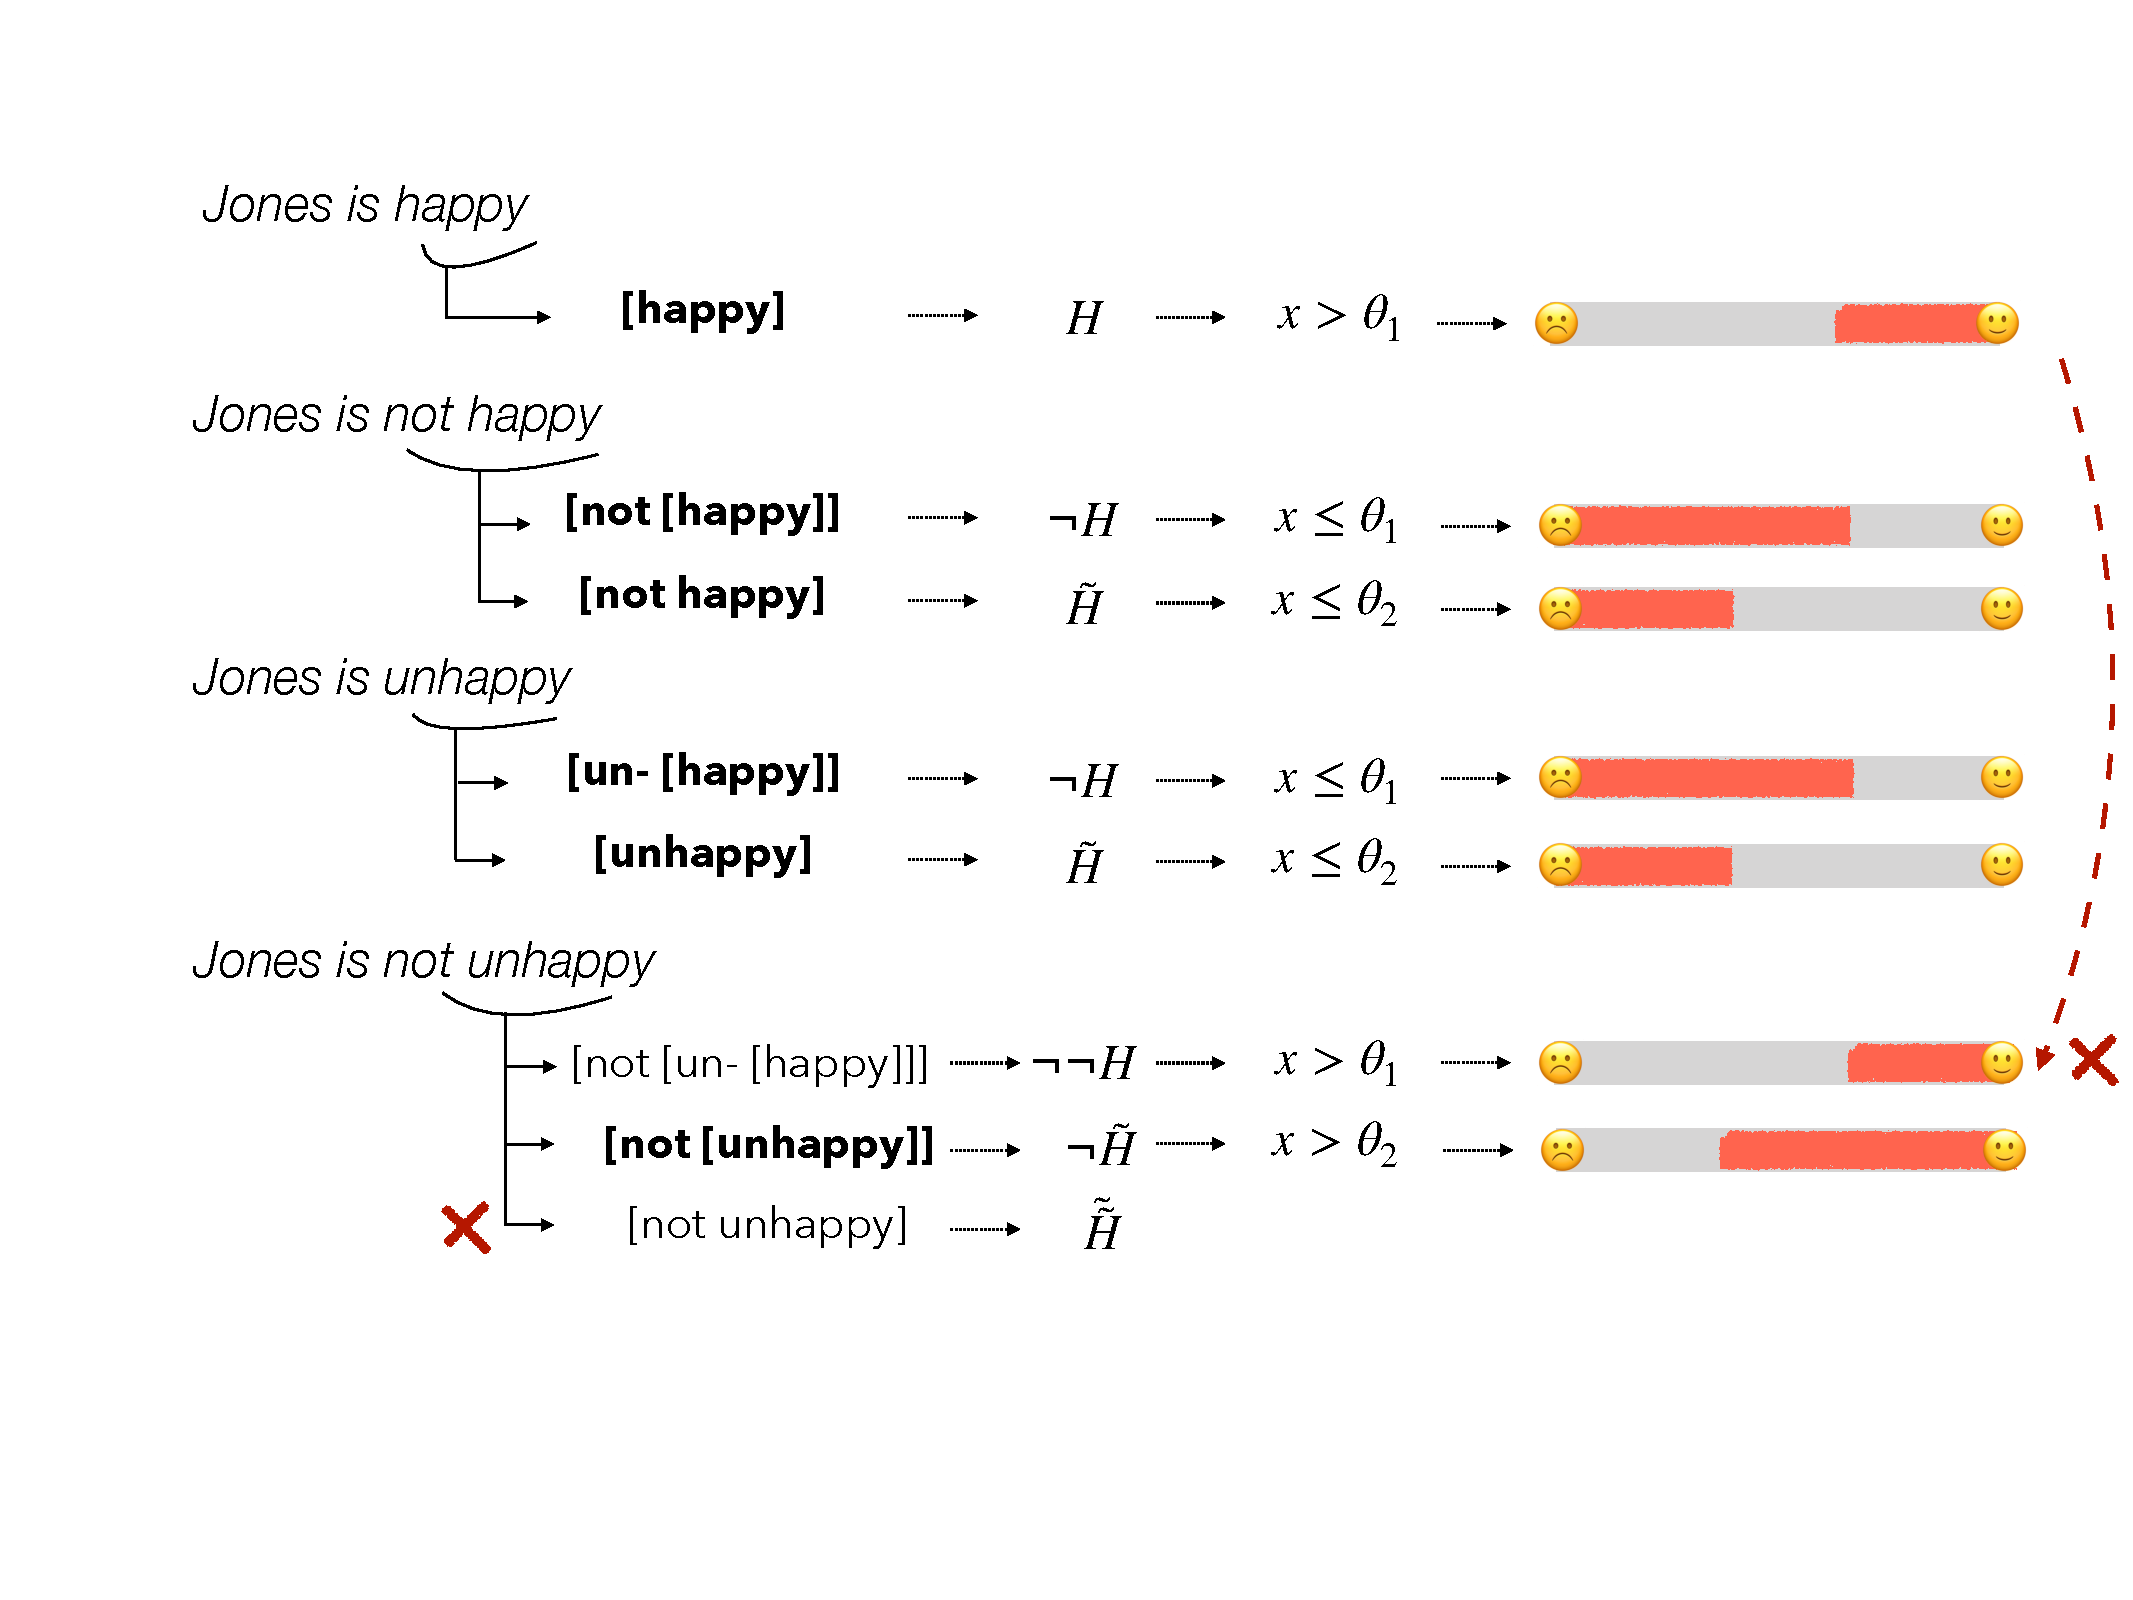
\includegraphics[width=0.8\textwidth]{figs/schematicMeanings}  
\caption{The \ourmodel model reasons over a hypothesis space of possible meanings for antonym pairs and their negations.
Both \emph{not happy} and \emph{unhappy} could signal either contradictory $\neg H$ or contrary negation $\tilde{H}$.
\emph{Not unhappy} can signal a double contradiction  $\neg \neg H$  or a contradiction of a contrary  $ \neg \tilde{H}$.
Contrary negation $\tilde{}$ cannot take wide scope over other negation operators (see SI). 
A double contradiction  $\neg \neg H$  is pragmatically unlikely, because the same meaning is expressed by just the simple positive $H$.
 Red bars denote the range of happiness values that are literally compatible with the adjective.
}
\label{fig:meanings}
\end{figure}

Complicating the question of semantic distinctions among negations is the fact that language understanding cannot unfold in a vacuum: The meanings of linguistics expressions manifest in communicative scenarios, which are subject to a host of pragmatic factors \cite{Grice1975, clark1996using, levinson2000presumptive}.
The fact that a speaker bothers to say that she's ``not happy''---and not, say, ``fine''---could imply that the speaker feels rather unhappy, a phenomenon referred to as \emph{negative strengthening} \cite{Horn1989:Natural, Blutner2004:pragmatics, benz2018scalar}.
On the other hand, a speaker could also say that she's ``unhappy'' (e.g., \citeNP{Krifka2007:Negated-antonyms}'s example above: ``I don't think I was \emph{unhappy}, just \emph{not happy}'').
Theorizing about the meanings of negation must consider how the communicative context supports and potentially alters meanings, but heretofore no formal models have been proposed that can adequately address the semantic question while also accounting for pragmatic reasoning.

We investigate the question of the meaning of natural language negation markers by formalizing the semantic proposals---Aristotelean, Orwellian, \ourmodel---in models of pragmatic communication that assume listeners interpret utterances as rational social actions taken by speakers \cite{FrankGoodman2014:Inferring-word-,FrankeScholler2016:Semantic-values}. 
Building on work in the Rational Speech Act framework, the basic architecture of these models is that a listener interprets an utterance like \emph{not unhappy} as being intentionally produced by a speaker (who could have produced alternative utterances, e.g., \emph{happy}) trying to communicate a degree of, say, happiness to the listener  \cite{Franke2015a, Goodman2016:RSA, problang}.
Our formal models of negation interpretation combine previous, independently established modeling proposals on pragmatic reasoning \cite{Goodman2016:RSA}, the interpretation of gradable adjectives \cite<e.g., \emph{tall}, \emph{happy};>{Kennedy2007, Lassiter2015}, and ambiguity in the meanings of words \cite{Bergen2016}. We describe the key qualitative differences of these models that lead to different predictions, but each model is supported by a completely formalized language understanding model, the mathematical details of which can be found in the SI. 
Each model takes in an utterance (e.g., \emph{not happy}, \emph{not unhappy}) and returns a posterior distribution on belief states concerning the degree of happiness (Figure \ref{fig:modelPredictions}), which we then qualitatively compare to empirical judgments in three experiments to determine which model most accurately characterizes the behavioral response patterns observed in human participants. 

The \ourmodel model predicts a pattern of data that is unique from that of the Aristotelean and Orwellian models and is context-dependent (Figure \ref{fig:modelPredictions}).
When utterances involving a single negation marker are heard in isolation (e.g., \emph{not happy} or \emph{unhappy}), they are interpreted identically \emph{a la} the Orwellian account because of the ambiguity in whether each maps onto a contrary or contradiction (Figure \ref{fig:meanings}).  
If the listener encounters a double negation (e.g., \emph{not unhappy}), however, pragmatic reasoning helps disambiguate that the speaker likely intended a contradiction of a contrary (\emph{a la} the Aristotelean account) because it would otherwise be a very costly manner of expressing the same meaning as the positive adjective (\emph{happy}), which would result from a double contradiction.
The disambiguating power of hearing multiple negations can also be observed for utterances with a single negation (\emph{not happy}, \emph{unhappy}) if the listener hears multiple distinct utterances in the same context (e.g., \citeNP{Krifka2007:Negated-antonyms}'s example, or more simply: ``She's not happy. He's unhappy.''; Figure \ref{fig:modelPredictions}, \emph{multiple utterances}). These indirectly contrastive inferences result from the fact that the listener has more evidence that the speaker associates different meanings with the different linguistic messages.
The \ourmodel model interprets the morphological antonym (\emph{unhappy}) as more strongly negative than the utterance involving a negation particle (\emph{not happy})  as a result of a cost difference between morphological and particle negation: we assume the production cost of morphology is less than that of particle negation because the speaker produces a one-word utterance as opposed to a two-word utterance.
We test these predictions in Experiments 1 \& 2.

%the meaning of a double negative like \emph{not unhappy}, while simultaneously showing no interpretative difference between the distinct single negations (\emph{not happy}~vs.~\emph{unhappy}) when heard in isolation (Figure \ref{fig:modelPredictions}, \emph{single utterances}). This model makes the additional prediction, though, that when several negation markers are heard in the same context 
%

% that listeners interpret double negatives as distinct from simple positives not because the negation markers have \emph{a priori} different meanings (as the Aristotelean analysis supposes), but because pragmatic reasoning---why would a speaker bother to use two distinct forms of negation?---can help disambiguate what is otherwise an uncertain hypothesis space of logical possibilities (Figure \ref{fig:meanings}).
% \footnote{
% Since contraries do not iterate, the \ourmodel hypothesis entertains that a double negative like \emph{not unhappy} could convey a double contradiction ($\neg \neg H$, like the Orwellian) or a contradiction about a contrary ($\neg \tilde{H}$, like the Aristotelean): The former carries the same meaning as $H$ (\emph{happy}) whereas the latter conveys a distinct meaning. 
% }


%Our \emph{\ourmodel} model's predictions are derived by reasoning about which meanings (contrary vs. contradiction) best explains a speaker's utterance (Figure \ref{fig:meanings}).
%Hearing multiple utterances by the same speaker, however, can provide the listener more information about how the speaker uses language,
%The formal modeling approach we take here naturally allows for this extension by simply providing the model with multiple adjective phrases; we condition each model on the observation of a speaker using all four adjective alternatives to describe different referents (e.g., \enquote{Sue is happy. Steve is not happy. Bill is unhappy. Barb is not unhappy.}; .
%Hearing multiple utterances has no effect on the Vanilla RSA model because it ascribes no uncertainty in meaning to the linguistic messages.
%All models derive more extreme differences in interpretations between utterances that could have different meanings (e.g., the difference between \emph{happy} and \emph{not unhappy} for \emph{Aristotle} is greater when it hears multiple utterances).
%Crucially, this inference results in the \emph{Tessler \& Franke} model predicting a meaning difference between \emph{unhappy} and \emph{not happy}: \emph{unhappy} is more negative than \emph{not happy}, producing the ordering hypothesized by \citeA{Krifka2007:Negated-antonyms} when both are used in the same context.



%produces a double-negation meant to do so in a non-redundant manner (i.e., \emph{not unhappy} means something different from \emph{happy}). 
%But unlike the Aristotelean hypothesis, this alternative hypothesis further predicts that \emph{not happy} and \emph{unhappy} inherit the same set of possible meanings, and thus two expressions are predicted to be interpreted in the same way (similar to the Orwellian analysis for \emph{not happy}~vs.~\emph{unhappy}).
%Intuitively, a rational speaker whose goal is to convey $H$ would avoid the double negative linguistic expression because it is more verbose than a simple positive utterance; thus, a listener could infer that a speaker who uses a double negative means to convey the expression with a unique meaning: a contradiction of a contrary, or $\neg \tilde{H}$.
%When a listener only hears a single negation marker (e.g., \emph{not happy} or \emph{unhappy}), the preference for either a contradictory or contrary meaning should disappear and thus, the two expressions are predicted to have the same interpretation (Figure \ref{fig:meanings}).


%To preview our findings, we find support for our \emph{\ourmodel} hypothesis across three experiments. 


Our \ourmodel hypothesis is not just an account of a few particular linguistic puzzles, but is a case study in how language users contort language to navigate and communicate the gradations of their conceptual landscape.
%Broadly, listeners rationalize utterances of speakers, especially when the utterances are unexpected \cite{Grice1975}.
%A listener who hears a double negation like \emph{not unhappy} looks for ways of rationalizing why the speaker has not used the simpler expression \emph{happy}.
The strongest form of this hypothesis as applied to negation is that the actual markers (\emph{not} \& \emph{un-}) are irrelevant to the reasoning and interpretation; all that need occur is that a speaker use two negation markers. 
In Experiment 3, we investigate the dependence on linguistic form by having participants interpret expressions that flagrantly use the same negation marker twice (e.g., \emph{not not happy}).
% in a way analogous to how they interpret negated antonyms that use distinct negation markers (e.g., \emph{not unhappy}). 
%Double negatives that flagrantly use the same negation marker twice are a strong test of the \ourmodel hypothesis, because 
In order to make sense of the utterance in a principled way, listeners would have to ascribe different meanings to the two different instances of \emph{not} (i.e., the utterance would indicate a contradiction of a contrary). 
%We investigate this possibility in Experiment 3.


\begin{figure}[h!]
\centering 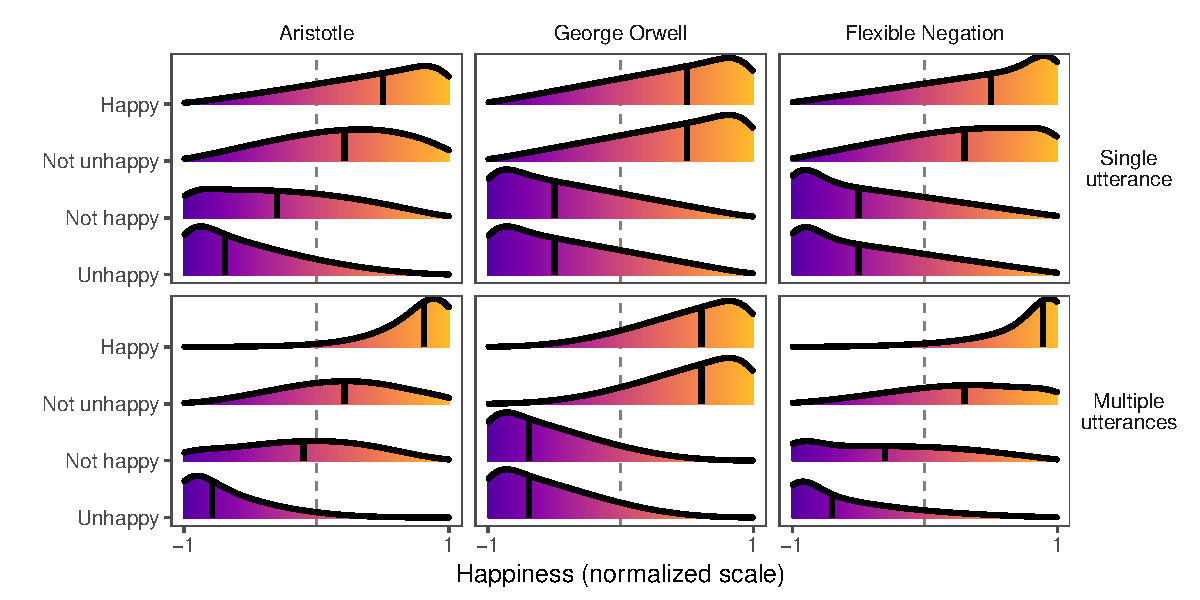
\includegraphics[width=\textwidth]{figs/alternativeModels_dists4.pdf} 
\caption{\small Model predictions for interpretations of antonym pairs and their negations under the three hypotheses. Black line shows the median of the distributions, in order to facilitate qualitative comparisons. \emph{Aristotle} draws a distinction between all adjective types both when the adjective is heard in isolation (single utterance) and when adjectives are heard in the same context (multiple utterances). \emph{George Orwell} never draws a meaning difference between the adjectives, even when they are heard in the same context. The \emph{\ourmodel} model generates a unique pattern of predictions:  When adjectives are heard in isolation, the model draws no difference in meaning between \emph{not happy} and \emph{unhappy} but does distinguish \emph{not unhappy} from \emph{happy}; when the adjectives are heard in the same context, the model distinguishes among all the adjectives. Dashed line denotes the mid-point of the scale. Model predictions use minimally assumptive model parameters described in the SI.}
%: $P(x) = \text{Uniform}(0, 1); \alpha = 1; \text{cost}(\mathit{un}) = 2; \text{cost}(\mathit{not}) = 3$.}.
\label{fig:modelPredictions}
\end{figure}

 

%Previous accounts have proposed both syntactic \cite{Cable2017} and pragmatic \cite{Rett2014:eval} mechanisms before, but heretofore there have been no formalized accounts tested against human behavioral data.





%If we find interpretations are analogous to negated antonyms which use distinct negation markers (e.g., \emph{not unhappy}), that would suggest that communicative reasoning can contort the basic logic of language 
%The \ourmodel hypothesis also raises questions about the boundary conditions of the flexibility: If even logical vocabulary, like negation markers, is prone to flexible interpretation, then what are its limits?
%Do human interlocutors interpret double negatives that flagrantly use the same negation marker twice (e.g., \emph{not not happy}) in a way analogous to how they interpret negated antonyms (e.g., \emph{not unhappy})?
%it is to be expected that speakers will also exploit this flexibility in speech production (e.g., by saying two things at once, as in the case of ``dog whistling'').
%Although we do not explore flexible language use from the speaker's point of view in this paper, the \ourmodel model would predict that speakers who want to say two things at once (e.g., speaking to two different audiences) can take advantage of this ambiguity to meet their personal communicative goals. 
%Pinning down the meanings of these simple linguistic expressions in a carefully controlled experimental setting, as we do below, will help map out the space of possible meanings available to speakers and listeners in the wild. 


%Might the contrary~vs.~contradiction distinction shed light on the meaning of double negatives?
%Indeed, this is the standard account: In an idealized, unidimensional space, the kinds of feelings associated with being \enquote{unhappy} are more negative than those associated with being \enquote{not happy} (Figure~\ref{fig:happy-scale}).
%Then, the meaning of \enquote{not unhappy} (a contradiction of a contrary) would partially overlap with the meaning of \enquote{happy}; a speaker who chooses to say \enquote{not unhappy} can then be judged to not have intended to convey that which could have been conveyed more succinctly by \enquote{happy} \cite{Horn1991:Duplex, Grice1975}.
%This logic, however, indicates only that \enquote{not unhappy} should not be taken to mean \emph{happy}; it doesn't imply that \enquote{not unhappy} indicates a slightly positive state, contra the intuition expressed by \citeA{Jespersen1924}.
%Is that intuition correct? 

%How does such a logical linguistic device---negation---give rise to a multiplicity of meanings?
%We imagine and resolve their uncertainty in context.  






%Like others (except perhaps George Orwell), we assume there are different kinds of negations and listeners are uncertain as to which kind of negation a speaker intends.
%We propose that two linguistic expressions conveying negation do not exactly cancel out because of an ambiguity at the heart of negation markers:
%In this paper, we 
%In addition, the ground truth as to the meaning of the language of negation has been left to the intuitions of trained theorists, who more often than not disagree on the basic facts. % come to different conclusions as to the meanings of these terms.




% the meaning of gradable adjectives like ``happy'' following standard semantic theories of gradable adjectives, wherein the adjective literally conveys that the associated degree of happiness is greater than some threshold $\theta$ \cite{Kennedy2007} but is interpreted in context in a fuzzy, or vague, manner by including uncertainty about what value the threshold should adopt \cite{Lassiter2015}.
%Uncertainty about the meaning of negation markers in the \emph{Uncertain Opposites} model follows the \emph{lexical uncertainty} technique of 
%
%To model the vagueness of adjectives like ``happy'', we adopt the technique of \citeA{Lassiter2015} that treats the 

%that human listeners are uncertain about the meaning of negation, and that rational, communicative reasoning can be used to derive subtle meanings in the moment. 
%We formalize this logic in a computational model building on the standard tools of formal semantics and probabilistic models of pragmatics 
%formalizes the uncertain opposites hypothesis as a case of \emph{lexical uncertainty} \cite{Bergen2016}. 









%We design experiments to test the four behavioral predictions that result from our \ourmodel model (Figure \ref{fig:modelPredictions}): (1.) Negated antonyms (\emph{not unhappy}) receive different interpretations than simple positives (\emph{happy}); (2.) Negated antonyms tend to receive a slightly positive interpretation (\emph{a la} \citeA{Jespersen1924}'s intuition above); (3.) Negated positives and morphological antonyms (\emph{not happy} and \emph{unhappy}) receive the same interpretation when presented in isolation; (4.) Negated positives and morphological antonyms receive different interpretations when presented in the same context. 
%%We test these predictions across three experiments using antonyms constructed by morphology (e.g., ``un-'' + adjective).
%We expect these predictions to apply to words with explicit negation markers (e.g., antonyms constructed by morphology such as \emph{un-} + \emph{happy}); as a control condition, we examine antonyms which do not have overt negation (e.g., \emph{tall} vs.~\emph{short}).
%Experiment 1 was exploratory and informed our computational modeling.
%Experiment 2 is a larger, more stringent, preregistered test of the four behavioral predictions outlined above.
%Finally, Experiment 3 interrogates how specific the patterns of inferences are to morphological negation (\emph{un-}) as opposed to negation more broadly by testing double negatives that use the same negation marker  (i.e., flagrant double negatives; e.g., \emph{not not happy}).






%A unique pattern of data is predicted by each of the models.
%By design, the \emph{George Orwell} model does not distinguish different kinds of negation, and a double negation like \enquote{not unhappy} returns the same distribution as the positive adjective (\enquote{happy}).
%When we hard-code different thresholds for \enquote{happy} and \enquote{unhappy} in the Vanilla RSA model, the model reasons that \enquote{not unhappy} does not communicate the same region of the space as \enquote{happy}; instead, the model restricts its interpretation to the neutral zone (i.e., \emph{not unhappy but not happy}); the same logic plays out for \enquote{not happy}, which receives the same neutral-feelings interpretation. 
%The model that represents the vagueness of an adjective like \enquote{happy} and treats \enquote{unhappy} as a \emph{bonafide contrary} predicts the intuitive ordering expressed by \citeA{Krifka2007:Negated-antonyms}: \emph{unhappy} $<$ \emph{not happy} $<$ \emph{not unhappy} $<$ \emph{happy}, with \emph{not unhappy} receiving a slightly positive interpretation.
%Finally, the full \ourmodel model predicts a different ordering: The \ourmodel model does not differentiate \enquote{unhappy} (antonyms) from \enquote{not happy} (negated positives), as \citeA{Jespersen1917:Negation} and \citeA{Blutner2004:pragmatics} surmised.
%At the same time, upon hearing \enquote{not unhappy}, the \emph{\ourmodel} model reasons that a truly compositional \(\neg \neg \textit{happy}\) is implausible because the speaker could have just said the simpler \enquote{happy} and
%interprets the utterance as signaling a slightly positive state (Fig.\(\thinspace\)\ref{fig:modelPredictions}).







%negation can mean two different things (i.e., there are different kinds of negation).
%\mht{check vanilla RSA with \ourmodel}
%of an interaction between and vagueness in meaning.

%such language could provide new avenues for understanding the language of emotions, like how it feels to be \emph{not unhappy} 
%Such a subtle, nonredundant meaning for double negatives (\emph{not} + \emph{un-}) is troubling from a formal perspective. 
%Negation is one of the basic logical elements of language and yet it seems to have the ability to step out of its logical cage.
%Understanding how double negations work can help clarify legal language, in which
%Moreover, a better understanding of such phenomena will provide deeper insight into how we manipulate and contort language to navigate and communicate the gradations of our conceptual landscape. 

%This intuition is not universally shared (cf., Orwell's quote above), nor is there consensus about why a listener should derive a weakly positive interpretation from a double negative.


%Any further interpretations 

%Little consensus is to be found in formal linguistics about why a listener should derive a weakly positive interpretation from a double negative.

%weaker than \enquote{happy}, not that it is necessarily positive. 


%Without further assumptions, however, this analysis predicts an interpretation of \enquote{not unhappy} as indicating neutral feelings (i.e., \emph{neither unhappy nor happy}), Further, the logic of communicative reasoning changes should a speaker consider producing \enquote{not happy}  though little agreement again is to be found on what \enquote{not happy} means (Figure~\ref{fig:happy-scale}B):
%Such an analysis, however, further depends on the meaning of \enquote{not happy} 
%The resulting pragmatic interpretation of \enquote{not unhappy} then depends upon how many other 
%
%
%resulting in a contextually strengthened interpretation corresponding to a neutral or indifferent state , contra \citeA{Jespersen1924}'s intuition that \enquote{not unhappy} is a slightly positive state.
%
%
%those of \enquote{not happy} and \enquote{unhappy} (\emph{negated positives} and \emph{antonyms}, respectively; Fig.\(\thinspace\)\ref{fig:happy-scale}; \citeNP{Krifka2007:Negated-antonyms}).



%\section{Modeling Double Negation}



% \(\neg \neg happy\) 
%The opposite of $(x > \theta_1)$ is either $(x \leq \theta_1)$ or $(x < \theta_2)$.
%.\footnote{
%Another example of iterated contradictory meaning is the intended meaning behind ``the enemy of my enemy is my friend''.
%} 
%With these basic facts, we provide an informal description of our model before moving onto its formal characterization.
 %\red{(e.g., there is no unshort)}.\% \cite{Horn1989:Natural}.
%QAs a result, a single negative (\enquote{not happy} and \enquote{unhappy}) can mean either \(\neg happy\) or \(\tilde{happy}\), while double negatives (\enquote{not unhappy}) may mean \(\neg \neg happy\) or \(\neg \tilde{happy}\) (Fig.\(\thinspace\)\ref{fig:lexicon-model}).}


%\mht{he}
%This hypothesis further predicts that a listener who hears only a single adjective phrase in isolation (e.g., \enquote{unhappy}) has no basis from which to decide whether a contrary or contradiction was intended, and thus the listener should impart no meaning difference between an isolated .
%and thus a rational speaker would not have bothered to say \emph{not unhappy} (a more complex expression) if a double contradiction was their intention, so they likely were contradicting a contrary.

%This mutual-exclusivity kind of reasoning is also predicted to occur were a speaker to use two distinct negations in the same context (e.g., \enquote{Jones is not happy, while Smith is unhappy}, also Krifka's example above); that is, the model predicts that \emph{unhappy} is intended to convey more negative feelings than \emph{not happy} when the model observes the speaker using both kinds of negation in the same context.
%Thus, hearing a double negation does provide sufficient evidence to the listener that the speaker intends two different kinds of negation. 
%\mht{do we want to say here that we are looking at the negation of scalar adjectives, as opposed to other negation like phenomena?}
%Then, interpreting negated antonyms of scalar adjectives like \enquote{not unhappy} involves not only reasoning about negation but how various kinds of negation interact with the vagueness of scalar adjectives like \emph{happy} or \emph{tall}.




%\mht{can we model this as an L2, where Lassiter adj model is modularized into $P(x \mid u, \mathcal{L})$ and we don't need to talk about thresholds?}
%\begin{align}
%P_L(x, \mathcal{L} \mid u) &\propto P_S(u \mid x, \mathcal{L}) \cdot P(x) \cdot P(\mathcal{L}) \\
%P_S(u \mid x, \mathcal{L}) &\propto \exp{(\alpha \cdot \ln {P(x \mid u, \mathcal{L})} - \text{cost}(u))} \label{eq:S1}
%\end{align}


%We hypothesize that \emph{lexical uncertainty}---uncertainty in the meaning of words---pervades even the language of logical devices, which interacts with conversational reasoning to give rise to a panoply of context-specific interpretations.
%Specifically, we posit that overt negation markers (\enquote{not}, \enquote{un-}) can convey different kinds of negation and that listeners resolve their uncertainty about the meaning in context.


%
%This formal model allows us to interrogate the conditions under which the above logic actually results in the interpretations we posit.
%%; it also allows us to understand the contribution of the vagueness of predicates like \enquote{happy} or \enquote{tall} (i.e., that there is no single threshold beyond which a person qualifies as tall). 
%Formally, a scalar adjective (e.g., \enquote{happy} or $H$) is thought to be literally true when the degree associated with that adjective \(x\) (e.g., the degree of happiness) is greater than some contextually-determined threshold \(\theta_1\): \(\mbox{ $[\![H]\!]$}(x, \theta_1): x > \theta_1\) \cite{Kennedy2007}.
%%If a negation marker (e.g., \enquote{not}) creates a 
%The contradictory opposite of such a meaning is simply that the degree is less than or equal to that same threshold: \( \mbox{ $[\![\neg H]\!]$}(x, \theta_1): x \leq \theta_1\).
%The contrary opposite, on the other hand, creates a new predicate, which for a gradable adjective takes the form of a function with its own, distinct threshold \(\theta_2\): \(\mbox{ $[\![ \tilde{H} ]\!]$}(x, \theta_2): x < \theta_2\).
%% which can in principle receive a different value than threshold $\theta_1$ for the positive adjective
%If listeners are uncertain about how \enquote{not} and \enquote{un-} map onto these logical meanings, then negated positives like \enquote{not happy} and morphological antonyms like \enquote{unhappy} could in principle take either meaning. 
%The hypothesis space of meanings for negated antonyms like \enquote{not unhappy} is constrained by the fact that contraries do not iterate; thus, negated antonyms either correspond to a double application of contradictory negation or a contradiction of a contrary.\footnote{``not un-H'' can then be either \(\neg \neg H\) or \(\neg (\tilde{H})\). Cashing these meanings out in terms of scalar adjectives, the order of operations need not matter: \(\neg (\tilde{H})\) $= \tilde{(\neg H)}$ , because both imply two sign-changes and one tokenization of a new threshold.}
%



%The act of producing a negated antonym (\enquote{not unhappy}) can then act as a signal towards the kinds of oppositions that the speaker had in mind (e.g., that the speaker intends to convey a contradictory negation of a contrary opposite).
%\mht{i think this point could be moved to a model implementation appendix or footnote}

%\red{Contradictory opposition can be iterated (\(\neg \neg Hx\)) but contrary opposition cannot \cite{Horn1989:Natural}.
%As a result, a single negative (\enquote{not happy} and \enquote{unhappy}) can mean either \(\neg happy\) or \(\tilde{happy}\), while double negatives (\enquote{not unhappy}) may mean \(\neg \neg happy\) or \(\neg \tilde{happy}\) (Fig.\(\thinspace\)\ref{fig:lexicon-model}).}
%
%%In order to generate predictions, 
%We embed these literal meanings in a probabilistic model of pragmatic reasoning, wherein a pragmatic listener $L_1$ resolves the meaning of an utterance $u$ by reasoning about why a rational speaker $S_1$ would have bothered to produce said utterance.
%Eqs.~\ref{eq:L0}--\ref{eq:L1} describe a recursive Bayesian model in the Rational Speech Act tradition \cite{Franke2015a, Goodman2016:RSA}, in which the listener  has additional uncertainty about how their interlocutor (speaker $S_1$) uses negation markers to convey contradictory~vs.~contrary negations \cite{Bergen2016}.
%We additionally take into account the vagueness of scalar adjectives using the technique proposed by \citeA{Lassiter2015} to derive thresholds \(\theta\) for interpreting vague adjectives (e.g., happy) in context:

%We formalize this as a prior distribution over possible lexica for the speaker $P(\mathcal{L})$.
%This model also takes into account the fact the scalar adjectives like \emph{happy} or \emph{tall} exhibit vagueness; i.e., there is no single, fixed $\theta$ beyond which the adjective is true. 
%---couched i---also a recursive reasoning model wherein a pragmatic listener \(L_{1}\) tries to resolve the intended meaning of an utterance \(u\) (e.g., \enquote{Jones is not unhappy}) by combining its prior beliefs about the degree of Jones' happiness \(P(x)\) with the Gricean assumption that speakers are generally cooperative \(S_1\) (Eqs.\(\thinspace\)\ref{eq:L1}-\ref{eq:L0}):
%Listener uncertainty about the interpretation of negation markers is modeled as uncertainty about the speaker's lexicon \(\mathcal{L}\) \cite{Bergen2016}.
%
%\vspace*{-0.5cm}
%
%\begin{align}
%L_{0}(x \mid u, \theta, \mathcal{L}) &\propto \mathcal{L}(u, x, \theta) \cdot P(x) \label{eq:L0} \\
%S_{1}(u \mid x, \theta, \mathcal{L}) &\propto \exp{(\alpha \cdot \ln {L_{0}(x \mid u, \theta, \mathcal{L})} - \text{cost}(u))} \label{eq:S1}\\
%L_{1}(x, \theta, \mathcal{L} \mid u) &\propto S_{1}(u \mid x, \theta, \mathcal{L}) \cdot P(x) \cdot  P(\theta) \cdot P(\mathcal{L}) \label{eq:L1}
%\end{align}
%
%The literal listener \(L_0\) (Eq. \ref{eq:L0}) updates their prior beliefs over the degree \(P(x)\) via an utterance's literal meaning in lexicon \(\mathcal{L}\),
%where \(\mathcal{L}(u, x, \theta)\) gives the truth-value of the utterance \(u\) in lexicon \(\mathcal{L}\) when applied to degree \(x\) (e.g., for $u= $\enquote{happy}, $\mathcal{L}$ returns a 1 when $x>\theta$ and a 0 when  $x\leq\theta$).
%The speaker (Eq.~\ref{eq:S1}) is a soft-max rational agent (with degree of rationality  $\alpha$) who aims to act in accordance with a standard, information-theoretic utility function that tracks how well an utterance conveys the speaker's intended meaning $x$ to this literal listener---$\ln {L_{0}(x \mid u, \theta, \mathcal{L}}$)---while taking into account the cost of the utterance---$\text{cost}(u)$.
%We assume that negation created by morphology (e.g., ``un-'' + happy) adds cost to the utterance as does creating a negation using the particle ``not'', and that the cost of ``un-'' is less than the cost of ``not''.\footnote{The \ourmodel model's qualitative predictions are sensitive to the exact values of the parameters. The predictions we show are invariant to cost so long as $\text{cost}(``un'') \leq \text{cost}(``not'')$ and $\alpha$ is relatively small. Our goal is to show, under intuitively plausible parameter values, the \ourmodel model has the capacity to the make the predictions we describe; none of the alternative models we articulate have the capacity to make the unique predictions of the \ourmodel model.}
%The intended meaning in this model is the value along a dimension referenced by an adjective (e.g., a degree of happiness).\footnote{
%	This meaning is a special case of modeling meaning as a probability distribution over degrees of happiness (e.g., the speaker has only a rough sense of their personal degree of happiness), in which case the speaker's utility would be a function of the KL divergence between the literal listener's prior and posterior distributions over the degree given the utterance. 
%}
%The pragmatic listener (Eq.~\ref{eq:L1}) interprets an utterance by reasoning about three variables: the intended meaning or degree $x$, the threshold beyond which a scalar adjective is literally true  $\theta$, and the speaker's lexicon \(\mathcal{L}\) describing how the speaker uses negation. 
%%, and the likelihood \(S_1(u \mid x, \theta, \mathcal{L})\) that a cooperative information-maximizing speaker would utter the adjective given a degree \(x\), threshold \(\theta\), and lexicon \(\mathcal{L}\).
%%The speaker model \(S_1\) (Eq.\ref{eq:S1}) describes an approximately rational agent (with degree of rationality \(\alpha\)) trying to inform a naive listener \(L_0\) about the degree \(x\).
%
%
%%\begin{figure}
%%\centering
%%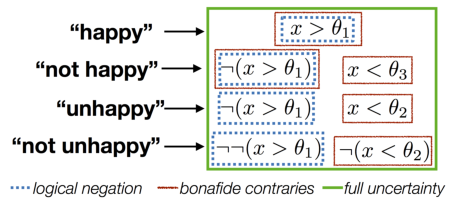
\includegraphics{figs/lexicon-model-1.pdf}
%%\caption{\label{fig:lexicon-model}Space of possible meanings in the lexicon prior for the \emph{logical negation}, \emph{bonafide contraries}, and the full \emph{\ourmodel} models.}
%%\end{figure}
%
%
%
%
%We compare the predictions of this \ourmodel model to three theoretically-interesting, simpler alternative models.
%First, we compare to a Vanilla RSA model which has neither lexical uncertainty about negation nor vagueness in the meaning of the adjective \cite{Frank2012}.\footnote{
%The vanilla model assumes fixed-thresholds to the adjectives, and we assume antonyms convey contrary meanings. Therefore, we ascribe the following meanings to the adjectives: \enquote{happy} means \(>70\%\) on the happiness scale; \enquote{unhappy} means \(<30\%\).
%}
%Second, we compare to the Vague RSA model of \citeA{Lassiter2015}, assuming that all negation markers entail contradictory negation (the \emph{logical negation} or \emph{George Orwell} model).
%Finally, we construct a \emph{bonafide contraries} model, building on \citeA{Lassiter2015}'s Vague RSA model by assuming morphological antonyms (\emph{un-}) convey contrary negation (e.g., \emph{unhappy} is to \emph{happy} how \emph{short} is to \emph{tall}) while the negation particular \emph{not} conveys contradictory negation.
%

%Finally, we construct fixed-threshold version of the \Ourmodel model: this model is a lexical uncertainty model in the style of \citeA{Bergen2016}, which differs from our \Ourmodel model only in its treatment of the semantics of the adjective as fixed as opposed to vague. 
%
%\begin{table}[t]
%\centering
%\begingroup\fontsize{10pt}{11pt}\selectfont
%\begin{tabularx}{\textwidth}{XXXXXXX}
%\toprule
%Model Name                    & Vagueness & Different negations & “happy”        & “un-”                            & “not ”                           \\ \midrule% & Description\\ \midrule
%Vanilla RSA                   & No        & Yes                         & $x > 0.7$      & $x < 0.3$                        & $x < 0.7$                        \\% & Hard-coded contraries and contradictions \\
%George Orwell                 & Yes       & No                          & $x > \theta$   & $x < \theta$                     & $x < \theta$                     \\% & Only Contradictions \\
%Bonafide Contraries & Yes       & Yes                         & $x > \theta_1$ & $x  < \theta_2$                  & $x < \theta_1$                   \\% & Contraries and Contradictions \\
%%Vanilla Lexical Uncertainty & No       & In Principle                         & $x > 0.7 $ & $x  < 0.3$ or   $x  < 0.7$              &  $x  < 0.3$ or   $x  < 0.7$                       \\% & Contraries and Contradictions \\
%\Ourmodel            & Yes       & In principle                & $x > \theta_1$ & $x  < \theta_2$ or $x < \theta_1$ & $x  < \theta_2$ or $x < \theta_1$ \\ %& Uncertain how “un” and “not” correspond with contrary vs. contradictory negation \\
%\bottomrule
%\end{tabularx}
%\endgroup
%\caption{Space of alternative models and the literal meanings they ascribe to negations.}
%\end{table}



% Please add the following required packages to your document preamble:
% \usepackage{booktabs}

%{]}
%--\textgreater{}
%This pattern of judgments is uniquely predicted by the \emph{\ourmodel} model.
%The \emph{bonafide contraries} model also yields interpretations of negated antonyms as slightly positive, but predicts that \enquote{unhappy} (morphological antonym) signals a more negative state than \enquote{not happy} (negated positive).
%The \emph{logical negation} model does not differentiate between negated antonyms and positives, nor between negated positives and antonyms.


%All models have more extreme interpretations when they condition on multiple utterances.



%\section{Overview of Experiments}
%
%The \emph{\ourmodel model} predicts a partial ordering for morphological antonyms and their negations when heard in isolation (with antonyms \(\approx\) negated positives), but a full ordering when present in the same context (Fig.\(\thinspace\)\ref{fig:modelPredictions}).
%As a control condition, we examine antonyms which do not have overt negation markers (e.g., \emph{short}).
%These lexical antonyms should behave as described by the \emph{Bonafide Contraries} model, which predicts a full ordering regardless of context.
%\text{Expt.$\thinspace$1} was exploratory and informed our computational modeling.
%\text{Expt.$\thinspace$2} is a larger, more stringent, preregistered (\url{osf.io/p7f25/}) replication.
%Finally, \text{Expt.$\thinspace$3} asks how specific the patterns of inferences are to morphological negation (\emph{un-}) as opposed to negation more broadly. 
%

\begin{table}[b]
\centering
\begingroup\fontsize{10pt}{11pt}\selectfont
\begin{tabularx}{\textwidth}{lll}
  \hline
 Adjective type & Definition & Examples \\ 
  \hline
 Positive & Positive-form scalar adjective & happy, mature \\ 
  Negated positive &  ``not'' + positive & not happy, not mature \\ 
  Morphological antonym &  Antonym created by morphology & unhappy, immature \\ 
  Lexical antonym & Antonym with a unique lexical item & sad, childish \\ 
  Negated morphological antonym &  ``not'' + morphological antonym & not unhappy, not immature \\ 
  Negated lexical antonym   &  ``not'' +  lexical antonym & not sad, not childish \\ 
  Negated negated positive (Expt.~3)  &  ``not'' + ``not'' + positive & not not happy, not not mature \\ 
   \hline
\end{tabularx}
\endgroup
\caption{Informal definitions and examples of adjective types investigated.} 
\end{table}

%\hypertarget{behavioral-experiments}




%\hypertarget{experiment-1-single-utterances}{%
%\subsection{Experiment 1: Single utterances}\label{experiment-1-single-utterances}
%}

\subsection{Methods}
%\hypertarget{participants}

We recruited 120 participants from Amazon's Mechanical Turk (MTurk).
This number was arrived at with the intention of getting approximately 25 ratings for each unique item in the experiment.
All experiments reported here required participants with U.S. IP addresses, at least 95\% work approval rating and English as a self-reported native language.
The experiment took on average 3 minutes and participants were compensated \$0.40.
%\rlgetnum{expt1_time_summary.csv}{}{}{aveTime}{0}

%\hypertarget{materials}

We used adjectives that described properties of people.
All of our adjectives were context-dependent, relative adjectives consistent with the definitions of \citeNP{Kennedy2007} and \citeNP{kennedy2005scale}.
We consider \emph{adjective sets} consisting of four related \emph{adjective types} (see Table~\ref{tab:Items}): positives (e.g., \emph{happy}, \emph{tall}), antonyms (e.g., \emph{short}, \emph{unhappy}), and their respective negations (\emph{not} X).

In addition to analyzing morphological antonyms, we test a control set of items consisting of \emph{lexical antonyms}, whose opposites are associated with distinct words (or, unique lexical items; e.g., \emph{tall} and \emph{short}). 
According to most theoretical proposals, these lexical antonyms should behave like bonafide contraries \emph{a la} the Aristotelean account, and we include these items to verify that our experimental methods are able to adequately detect the behavioral signature associated with contraries. 
That is, we expect the lexical antonyms to behave according the Aristotelean model.
% Antonyms can be either lexical (\emph{short}) or morphological (\emph{unhappy}).
In total, twenty adjective sets were constructed, ten for lexical antonyms (\emph{short}) and ten for morphological antonyms (\emph{unhappy}). 
%\mf{I removed the following information, because it doesn't seem to be very important for the goal of understanding the set-up and/or making the paper stronger: ``from an informal survey of the linguistics literature and taken from a list of \enquote{common opposites} available online . Footnote: \url{http://www.enchantedlearning.com/wordlist/opposites.shtml}''.}

\begin{table}[h]
\centering
\begingroup\fontsize{10pt}{11pt}\selectfont
\begin{tabular}{ll}
  \hline
Morphological antonyms & Lexical antonyms \\ 
  \hline
attractive, unattractive & beautiful, ugly \\ 
  educated, uneducated & brave, cowardly \\ 
  friendly, unfriendly & fat, skinny \\ 
  happy, unhappy & hard-working, lazy \\ 
  honest, dishonest & loud, quiet \\ 
  intelligent, unintelligent & proud, humble \\ 
  interesting, uninteresting & rich, poor \\ 
  mature, immature & strong, weak \\ 
  polite, impolite & tall, short \\ 
  successful, unsuccessful & wise, foolish \\ 
   \hline
\end{tabular}
\endgroup
\caption{Items in Experiment 1.}
\label{tab:Items}
\end{table}


%\hypertarget{procedure}

On each trial, participants read a statement introducing a person using a gradable adjective of one of four \emph{adjective types} from one of the two sets of \emph{antonym types} (lexical vs. morphological) described in Materials. 
% positives (e.g., \emph{happy}, \emph{tall}), antonyms (e.g., \emph{short}, \emph{unhappy}), and their respective negations (\emph{not} X).
%Antonyms were one of two types: morphological (e.g., \emph{unhappy}) and lexical (e.g., \emph{short}).
Participants rated the character on a scale from \enquote{the most \emph{positive} person} to \enquote{the most \emph{antonym} person} (item-dependent) using a slider bar (Fig.$\thinspace$\ref{fig:experiment-slides}A).
Participants rated one sentence at a time and saw items from both antonym types throughout the experiment.
Each participant completed a total of 16 trials, with exactly 2 repetitions of each adjective type for each antonym type.
No participant saw two instances from the same adjective set.


\begin{figure}[bt]
{\centering 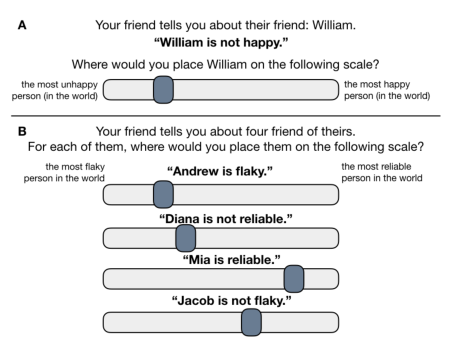
\includegraphics[width=0.7\linewidth]{figs/experiment-slides-1} 

}
\caption{Example experimental trials for (A) single utterance (Expts.~1, 2) and (B) multiple utterances (Expts.~2, 3) conditions. ``in the world'' wording for endpoints was used in Expts.~2 \& 3. (A) shows a trial from a morphological antonym set while (B) shows a lexical antonym set.}\label{fig:experiment-slides}
\end{figure}

\begin{figure}[h]
\centering 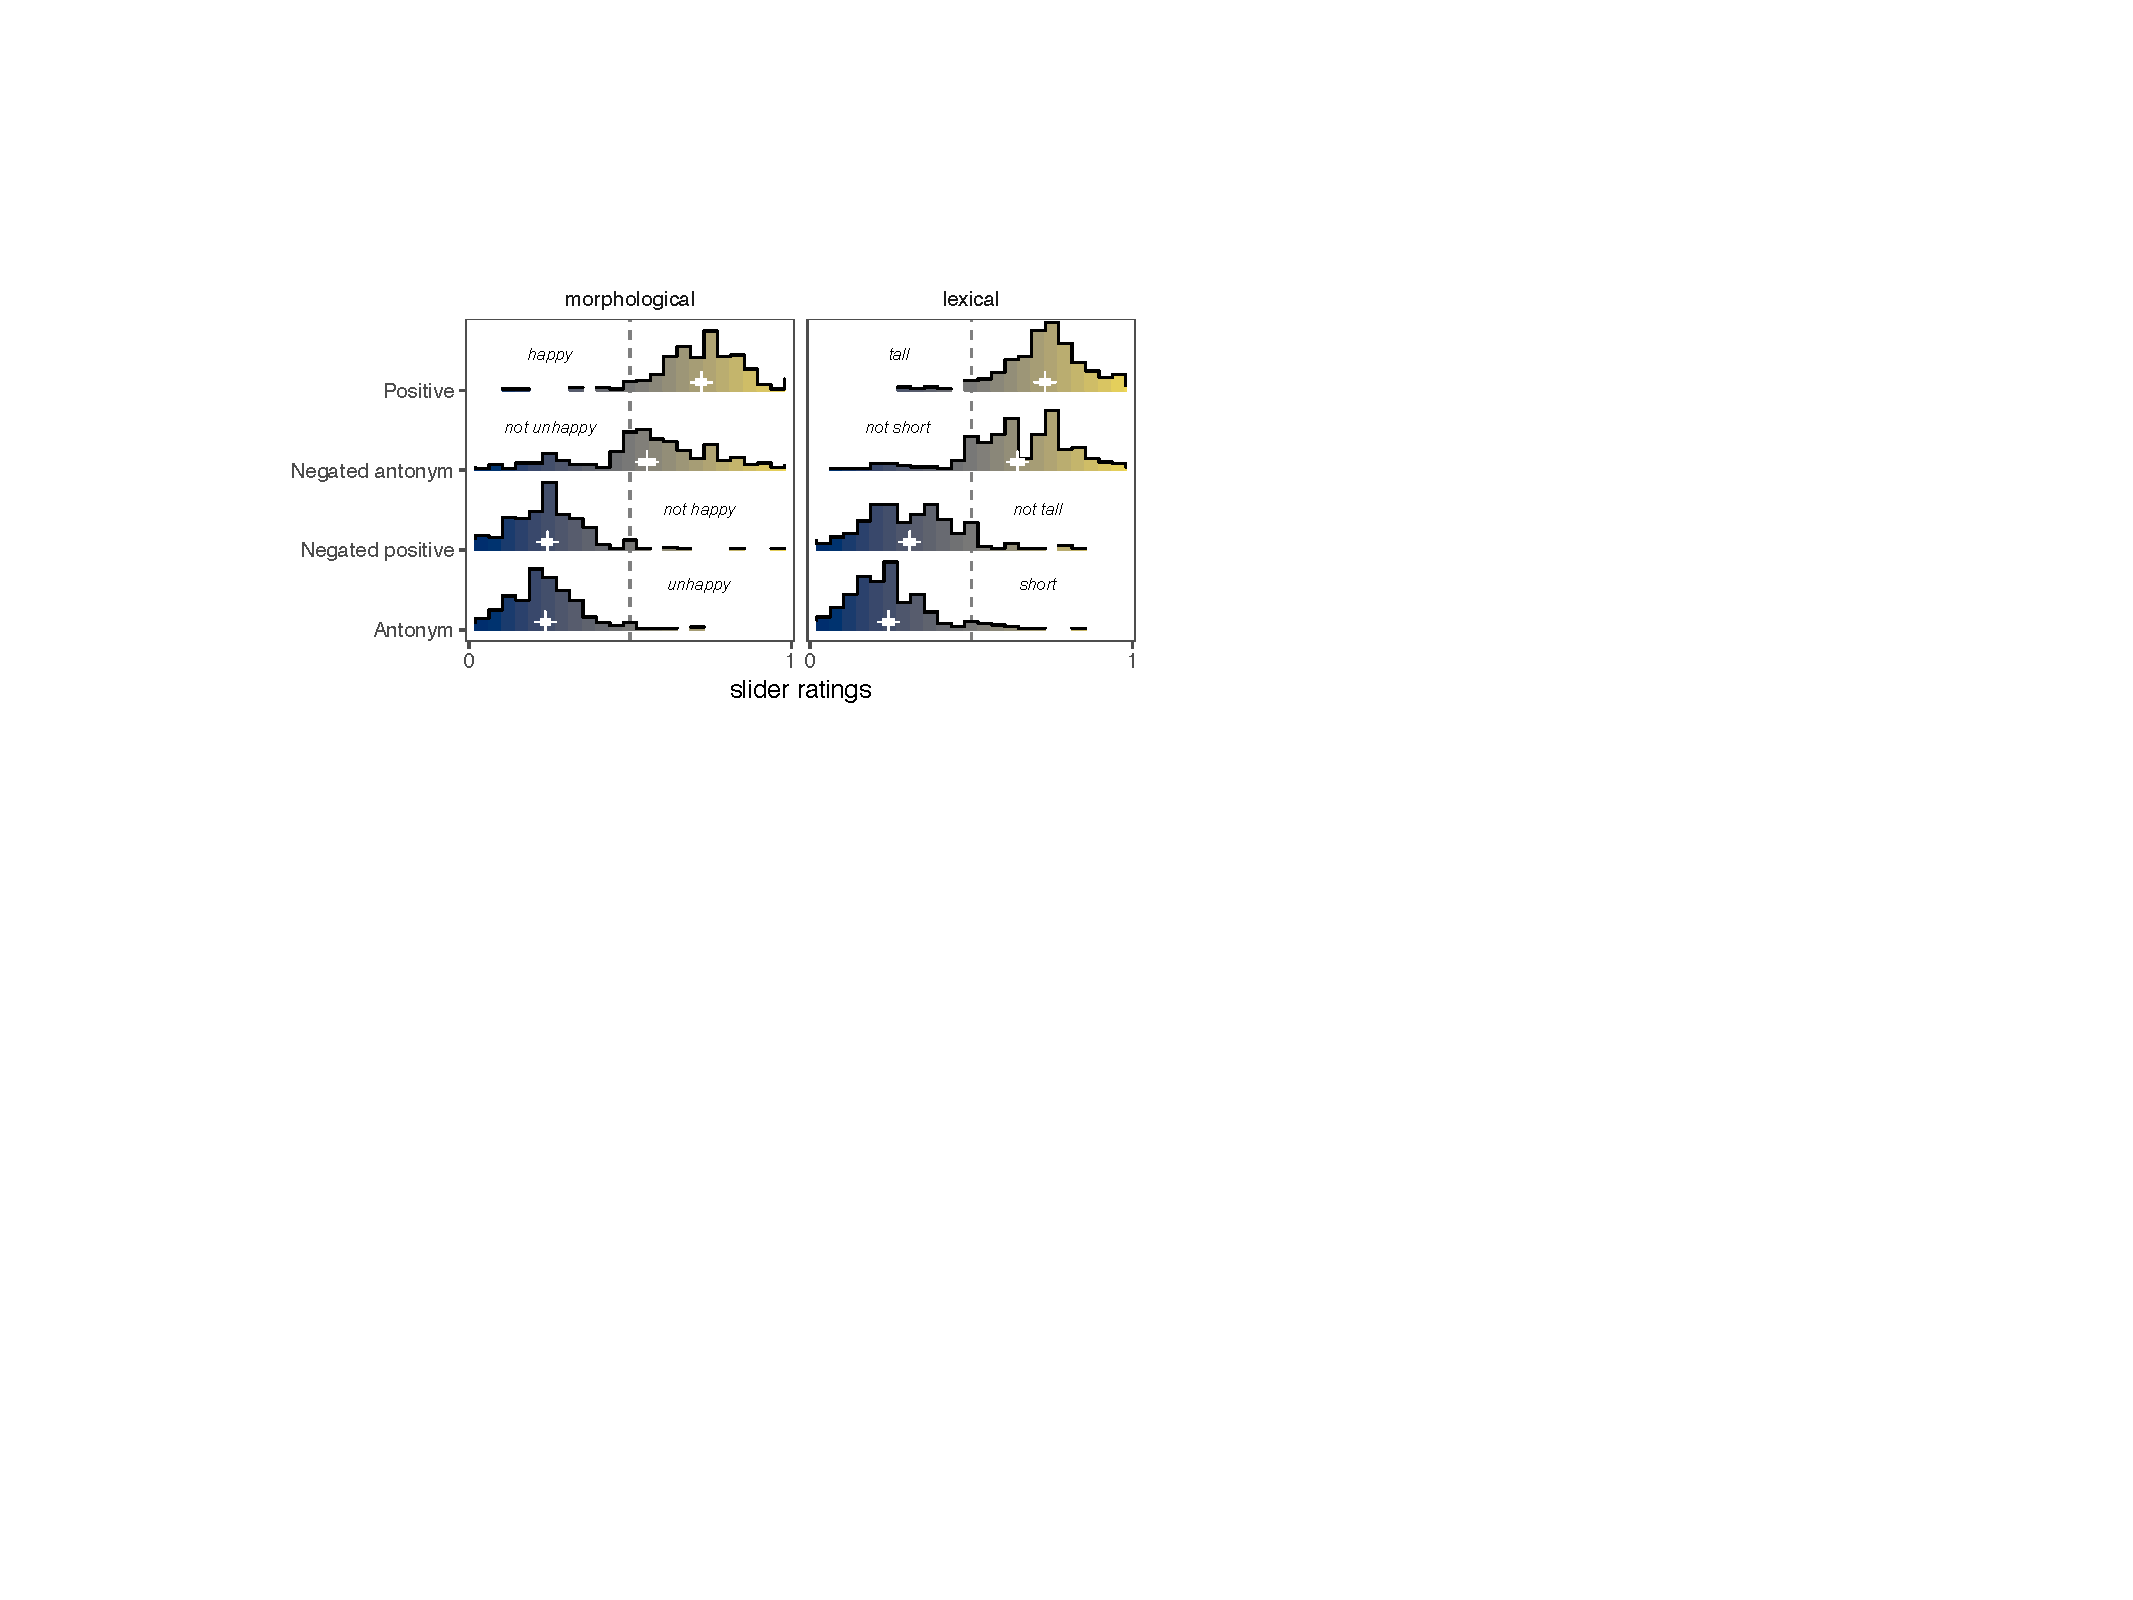
\includegraphics[width=0.95\linewidth]{figs/expt1_directlabel_hist} 
\caption{ Experiment 1 results. Empirical histograms of responses for adjective sets with morphological antonyms (e.g., \emph{happy/unhappy}) and lexical antonyms (e.g., \emph{tall/short}). Dashed line indicates the midpoint of the scale.  White bars denote bootstrapped 95\% confidence intervals for the means.}\label{fig:expt1-results}
\end{figure}
%\hypertarget{results}

Six participants were excluded for self-reporting a native language other than English, leaving a remainder of 114 participants for these analyses, which resulted in an average of 23 ratings for each unique adjective in our stimulus set.
The qualitative predictions of our models concern the ordering within a set of alternatives for different antonym types (morphological vs.~lexical).
%To visualize the data, we compute normalized responses on a participant-wise basis (i.e., normalized response \(r'_{ij} = \frac{r_{ij} - mean_j}{sd_j}\) for trial \(i\) and participant \(j\)).
Figure \ref{fig:expt1-results} shows the empirical distributions for each of the four adjective types for both morphological and lexical antonyms adjective sets.
Critically, as predicted by the \ourmodel model, adjective sets with morphological antonyms show only a partial ordering, with negated positives (e.g., \emph{not happy}) and morphological antonyms (e.g., \emph{unhappy}) receiving the same ratings; at the same time, the adjective sets with lexical antonyms show a full ordering (i.e., all adjective types receive distinct interpretations).

To confirm these observations, we built a Bayesian generalized linear mixed model predicting the raw ratings in terms of fixed effects of \emph{antonym type} (morphological vs.~lexical), \emph{adjective type}, %\footnote{Forward difference coding compares adjacent-levels of a factor, which allows for the following comparisons: antonym vs.~negated positive, negated positive vs.~negated antonym, negated antonym vs.~positive.}, 
and their interaction; the model included a maximal random-effects structure with random intercepts, slopes of \emph{adjective type}, \emph{antonym type}, and their interaction, by-participant and by-item.\footnote{All regression models use a ``zero-, one- inflated Beta'' linking function which models data on the [0, 1] interval, using the \texttt{brms} package in R \cite{brms}.} %the maximal mixed-effects model that converged for the data set that additionally explained significantly more variance than models with simpler mixed-effects structures, using the \texttt{lme4} package in R \cite{lme4}.
%}
Consistent with our predictions, the difference between the \emph{antonym} vs.~\emph{negated positive} 
%\mf{this is comparing a factor to a factor level; we should say what the coding scheme is, if applicable what the default level is and then write something like \emph{lexical} vs~\emph{negated positive}, right?}
levels of adjective type interacted with the morphological~vs.~lexical antonym type (posterior mean and 95\% Bayesian credible interval: \brmresultsp{expt1_brm_contrasts_10k.csv}{int_lex_morph_ant_v_negpos}; Cohen's $d$ effect size: \effsize{expt1_brm_effsize_10k.csv}{int_lex_morph_ant_v_negpos}).\footnote{We compute effect sizes by following the Bayesian technique described in \cite{kruschke2014doing} Ch.~16. See SI for details.}.
% (morphological vs. lexical; standardized regression coefficients \(\beta = \rlgetnum{expt1_norm_helmert_summary.csv}{Rowname}{antonym_typelexical:adjective_type1}{Estimate}{3}\), SE = 
%\rlgetnum{expt1_norm_helmert_summary.csv}{Rowname}{antonym_typelexical:adjective_type1}{Std..Error}{3},
%t\((\rlgetnum{expt1_norm_helmert_summary.csv}{Rowname}{antonym_typelexical:adjective_type1}{df}{0}) = \rlgetnum{expt1_norm_helmert_summary.csv}{Rowname}{antonym_typelexical:adjective_type1}{t.value}{2}, p = \rlgetnum{expt1_norm_helmert_summary.csv}{Rowname}{antonym_typelexical:adjective_type1}{Pr...t..}{3}\)) such that the difference between negated positives and antonyms was stronger for lexical antonyms than morphological antonyms.
The negated positive vs. antonyms contrast (e.g., \emph{unhappy} vs. \emph{not happy}) was not appreciably different for the morphological antonyms (\brmresultsp{expt1_brm_contrasts_10k.csv}{morph_ant_v_negpos}; \effsize{expt1_brm_effsize_10k.csv}{morph_ant_v_negpos}), but with lexical antonyms (e.g., \emph{short} vs. \emph{not tall}), this difference was non-zero (\brmresultsp{expt1_brm_contrasts_10k.csv}{lex_ant_v_negpos}; \effsize{expt1_brm_effsize_10k.csv}{lex_ant_v_negpos}). %(e.g., \emph{unhappy} vs. \emph{not happy}; \(\beta = \rlgetnum{expt1_norm_helmert_summary.csv}{Rowname}{adjective_type1}{Estimate}{3}\), SE = 
%\rlgetnum{expt1_norm_helmert_summary.csv}{Rowname}{adjective_type1}{Std..Error}{3}, t\((\rlgetnum{expt1_norm_helmert_summary.csv}{Rowname}{adjective_type1}{df}{0}) = \rlgetnum{expt1_norm_helmert_summary.csv}{Rowname}{adjective_type1}{t.value}{2}, p = \rlgetnum{expt1_norm_helmert_summary.csv}{Rowname}{adjective_type1}{Pr...t..}{3}\)).
%Running the same model with the antonym type coded with lexical antonyms as the default level reveals that the negated positive vs. antonyms contrast was significantly different for the lexical antonyms (e.g., \emph{short} vs. \emph{not tall}; \(\beta = \rlgetnum{expt1_norm_helmert_summary_lexBase.csv}{Rowname}{adjective_type1}{Estimate}{3}\), SE = 
%\rlgetnum{expt1_norm_helmert_summary_lexBase.csv}{Rowname}{adjective_type1}{Std..Error}{3}, t\((\rlgetnum{expt1_norm_helmert_summary_lexBase.csv}{Rowname}{adjective_type1}{df}{0}) = \rlgetnum{expt1_norm_helmert_summary_lexBase.csv}{Rowname}{adjective_type1}{t.value}{2}, p = \rlgetnum{expt1_norm_helmert_summary_lexBase.csv}{Rowname}{adjective_type1}{Pr...t..}{3}\)).
%\mf{double-check if this is right: $\beta$ estimate and $p$ accidentally receive the same value?} \mf{Double-CheckL: reporting a significant interaction (even if in the right direction) might not enough for the conclusions we want to draw from this. If \emph{antonym type} is dummy-coded with default \emph{morhpological}, we'd need to report significance of at least the first Helmert-contrast, right?}
 

%","Estimate"],3)`$,  t$(`r round(rs1.expt1.coef["antonym_typelexical:st1","df"], 1)`) = `r round(rs1.expt1.coef["antonym_typelexical:st1","t value"],2)`, p = `r round(rs1.expt1.coef["antonym_typelexical:st1","Pr(>|t|)"], 3)`$).

We observe further that negated morphological antonyms (e.g., \emph{not unhappy}) were rated differently and lower than positive adjectives (\brmresultsp{expt1_brm_contrasts_10k.csv}{lex_ant_v_negpos}; \effsize{expt1_brm_effsize_10k.csv}{lex_ant_v_negpos}). %(e.g., \emph{happy}; \(\beta = \rlgetnum{expt1_norm_helmert_summary.csv}{Rowname}{adjective_type3}{Estimate}{3}\), SE =  \rlgetnum{expt1_norm_helmert_summary.csv}{Rowname}{adjective_type3}{Std..Error}{3}, t\((\rlgetnum{expt1_norm_helmert_summary.csv}{Rowname}{adjective_type3}{df}{0}) = \rlgetnum{expt1_norm_helmert_summary.csv}{Rowname}{adjective_type3}{t.value}{2}, p <0.001\)). 
We additionally observe that negated morphological antonyms (e.g., \emph{not unhappy}) were rated overall lower than negated lexical antonyms (e.g., \emph{not tall}; Figure \ref{fig:expt1-results}), which manifested as an interaction in the negated antonym vs. positive contrast with the lexical vs. morphological items (\brmresultsp{expt1_brm_contrasts_10k.csv}{int_lex_morph_negant_v_pos};  \effsize{expt1_brm_effsize_10k.csv}{int_lex_morph_negant_v_pos}). 
%(\(\beta = \rlgetnum{expt1_norm_helmert_summary.csv}{Rowname}{antonym_typelexical:adjective_type3}{Estimate}{3}\), SE = 
%\rlgetnum{expt1_norm_helmert_summary.csv}{Rowname}{antonym_typelexical:adjective_type3}{Std..Error}{3},  t\((\rlgetnum{expt1_norm_helmert_summary.csv}{Rowname}{antonym_typelexical:adjective_type3}{df}{0}) = \rlgetnum{expt1_norm_helmert_summary.csv}{Rowname}{antonym_typelexical:adjective_type3}{t.value}{2}, p = \rlgetnum{expt1_norm_helmert_summary.csv}{Rowname}{antonym_typelexical:adjective_type3}{Pr...t..}{3}\)).
Negated antonyms received a distinct bimodal distribution wherein most ratings were slightly positive but a minority distribution of ratings were slightly negative (e.g., \emph{not dishonest} meaning \emph{not honest}).
This weakly negative interpretation for negated antonyms was present at least somewhat in every item and in most participants.
This interpretation may be the result of participants attributing politeness to the speaker; when speakers care about a listener's self-image, human participants tend to endorse utterances with negation:  \emph{Not dishonest} may be an indirect way of saying that a person is not honest \cite{Yoon2017}.

While we note the differences between lexical and morphological antonyms in this experiment, the direct comparison of these two kinds of adjectives is difficult. 
We have coded the antonyms in the morphological sets as positive and negative (or, antonym) by appealing to the morphology (e.g., \emph{happy} is the positive adjective, while \emph{unhappy} is the antonym); a similar assignment of the lexical antonyms to positive and negative is not always possible.
Some pairs have a clear unmarked form: \emph{tall} is the positive adjective because when describing the height of a person, we say \emph{six feet tall} and not \emph{six feet short}.
For items that did not have a clear unmarked form (e.g., \emph{fat} and \emph{skinny}), we assigned the adjective that conveyed a greater amount to be the positive (i.e., fat conveys more weight than skinny); thus, the positive adjective is not necessarily the socially more desirable feature.\footnote{
In addition, in the empirical data, we see a bimodal distribution of responses for the negated lexical antonyms and negated positives; thus, one may be concerned that this bimodal distribution is the result of an improper assignment of lexical antonyms to either the positive or antonym form (e.g., \emph{skinny} is actually the positive adjective and \emph{fat} is the antonym). 
If this were so, we would expect this bi-modality to occur across the items but not within items; however, when we look at the item-specific distributions of responses, we do not see clear evidence for this, but rather we see the bi-modality occurring within several items from the lexical sets (see SI).
}
Because of these differences between lexical and morphological antonym sets, we treated this experiment as exploratory and curated a more tightly controlled set of materials for Experiments 2 \& 3.



%\hypertarget{experiment-2-single-and-multiple-utterances}

%\text{Experiment$\thinspace$1} revealed an asymmetry: Lexical antonyms (e.g., \emph{short}) were distinguished from negated positives (e.g., \emph{not tall}), whereas morphological antonyms were not (e.g., \emph{unhappy} \(\approx\) \emph{not happy}).
%In \text{Experiment$\thinspace$1}, our adjective sets varied both in terms of their antonym type (morphological vs.\text{~}lexical) as well as the actual degree scales being described (e.g., height for \emph{tall}/\emph{short} vs.\text{~}happiness for \emph{happy}/\emph{unhappy}).
%Many adjective sets have both morphological and lexical antonyms (e.g., \emph{happy}/\emph{unhappy}/\emph{sad}).

We aim to replicate the previous findings using adjectives that describe the same semantic scales (e.g.,  \emph{happy}~vs.~\emph{unhappy}~vs.~\emph{sad}).
Also, we test our second prediction that hearing multiple utterances in the same context will produce the full ordering for morphological antonym sets (Fig.\(\thinspace\)\ref{fig:modelPredictions}).

\subsection{Methods}
%\hypertarget{participants-1}

We recruited 750 participants from MTurk.
The experiment comprised four between-subjects experimental conditions arranged in a 2x2 design: \emph{antonym type} (morphological vs.~lexical) X \emph{context} (single vs.~multiple utterances).
Three-hundred participants were assigned to each \emph{antonym type} in the \emph{single utterance} contexts, and 75 participants were assigned to each in the \emph{multiple utterances} conditions.
These numbers follow from the intention of getting approximately 45 ratings for each unique adjective in the experiment.
The \emph{single utterance} task took on average 3 minutes and participants were compensated \$0.40; \emph{multiple utterances} took on average 5 minutes and participants were compensated \$0.80.
Exclusion criterion, sample size, procedure, and the analysis described below were preregistered: \url{osf.io/p7f25/}.

%\hypertarget{materials-1}

To best isolate the contribution of morphological vs.\text{~}lexical antonyms, we curated adjective sets consisting of words for properties of people, such that both types of antonyms existed for the same positive adjective (e.g., \emph{happy} \(\rightarrow\) \emph{unhappy}, \emph{sad}; \text{Table 4}).
Lexical antonyms were selected from a set of possibilities produced from a small survey (n=18) on MTurk eliciting \enquote{opposites} for a list of thirty positive-form adjectives which had morphological antonyms.
In this antonym elicitation, participants saw the same material as in the main experiment (e.g., ``Your friend tells you about their friend: William. \emph{William is forgiving.}'') and asked \enquote{What is the opposite of \emph{adjective}?} (e.g., ``What is the opposite of forgiving?'').
From the list of freely-produced opposites, the first author chose the one that intuitively best conveyed the same scalar dimension as the morphological antonym and which was not already used as a lexical antonym for another item (e.g., opposite of \emph{forgiving} \(\rightarrow\) \emph{resentful}; opposite of \emph{kind} \(\rightarrow\) \emph{cruel}, because opposite of \emph{friendly} \(\rightarrow\) \emph{mean}).
Ten out of the original thirty items were dropped for either not having such a well-suited lexical antonym (e.g., \emph{moral}) or for having a well-suited lexical antonym that conflicted with another item (e.g., \emph{compassionate} \(\rightarrow\) \emph{cold}, but also \emph{affectionate} \(\rightarrow\) \emph{cold}).

%\hypertarget{procedure-1}

In the \emph{multiple utterances} conditions, participants rated all four adjective types simultaneously, each referring to a different person (Fig.$\thinspace$\ref{fig:experiment-slides}B), for a total of 12 trials.
The \emph{single utterances} conditions were similar to that of \text{Experiment$\thinspace$1}: Participants rated one sentence at a time (e.g., \enquote{Greg is not unhappy}), each from a unique adjective set (e.g., never rated both \emph{unhappy} and \emph{not happy}), completing a total of 12 trials, with exactly 3 repetitions of each adjective type (positive, antonym, and their negations).
In contrast to \text{Experiment$\thinspace$1}, \emph{antonym type} (morphological vs.\text{~}lexical) was a between-participants factor.
In addition, the slider bar endpoints were relabeled to \enquote{the most \{\emph{positive}, \emph{negative}\} person \emph{in the world}}; without \enquote{in the world}, there is a salient interpretation of the endpoints as \enquote{the most \{\emph{positive}, \emph{negative}\} person (of these four)} in the multiple utterances conditions.
We note that by labelling the endpoints in this more explicit manner, we potentially decrease the size of the effects we observe 

\begin{table}[h]
\centering
\begingroup\fontsize{9pt}{10pt}\selectfont
\begin{tabular}{lll}
  \hline
Positive adjective & Morphological antonym & Lexical antonym \\ 
  \hline
affectionate & unaffectionate & cold \\ 
  ambitious & unambitious & lazy \\ 
  attractive & unattractive & ugly \\ 
  educated & uneducated & ignorant \\ 
  forgiving & unforgiving & resentful \\ 
  friendly & unfriendly & mean \\ 
  generous & ungenerous & stingy \\ 
  happy & unhappy & sad \\ 
  honest & dishonest & deceitful \\ 
  intelligent & unintelligent & stupid \\ 
  interesting & uninteresting & boring \\ 
  kind & unkind & cruel \\ 
  mature & immature & childish \\ 
  patriotic & unpatriotic & traitorous \\ 
  polite & impolite & rude \\ 
  rational & irrational & crazy \\ 
  reliable & unreliable & flaky \\ 
  resourceful & unresourceful & wasteful \\ 
  sincere & insincere & fake \\ 
  tolerant & intolerant & bigoted \\ 
   \hline
\end{tabular}
\endgroup
\caption{Items used in Experiment 2.} 
\end{table}

%\hypertarget{results-1}

Thirty-five participants were excluded for self-reporting a native language other than English, leaving 715 participants for these analyses.
Results for each adjective type in each condition are shown in Fig.$\thinspace$\ref{fig:expt2-results}.


\begin{figure}[t]
\centering 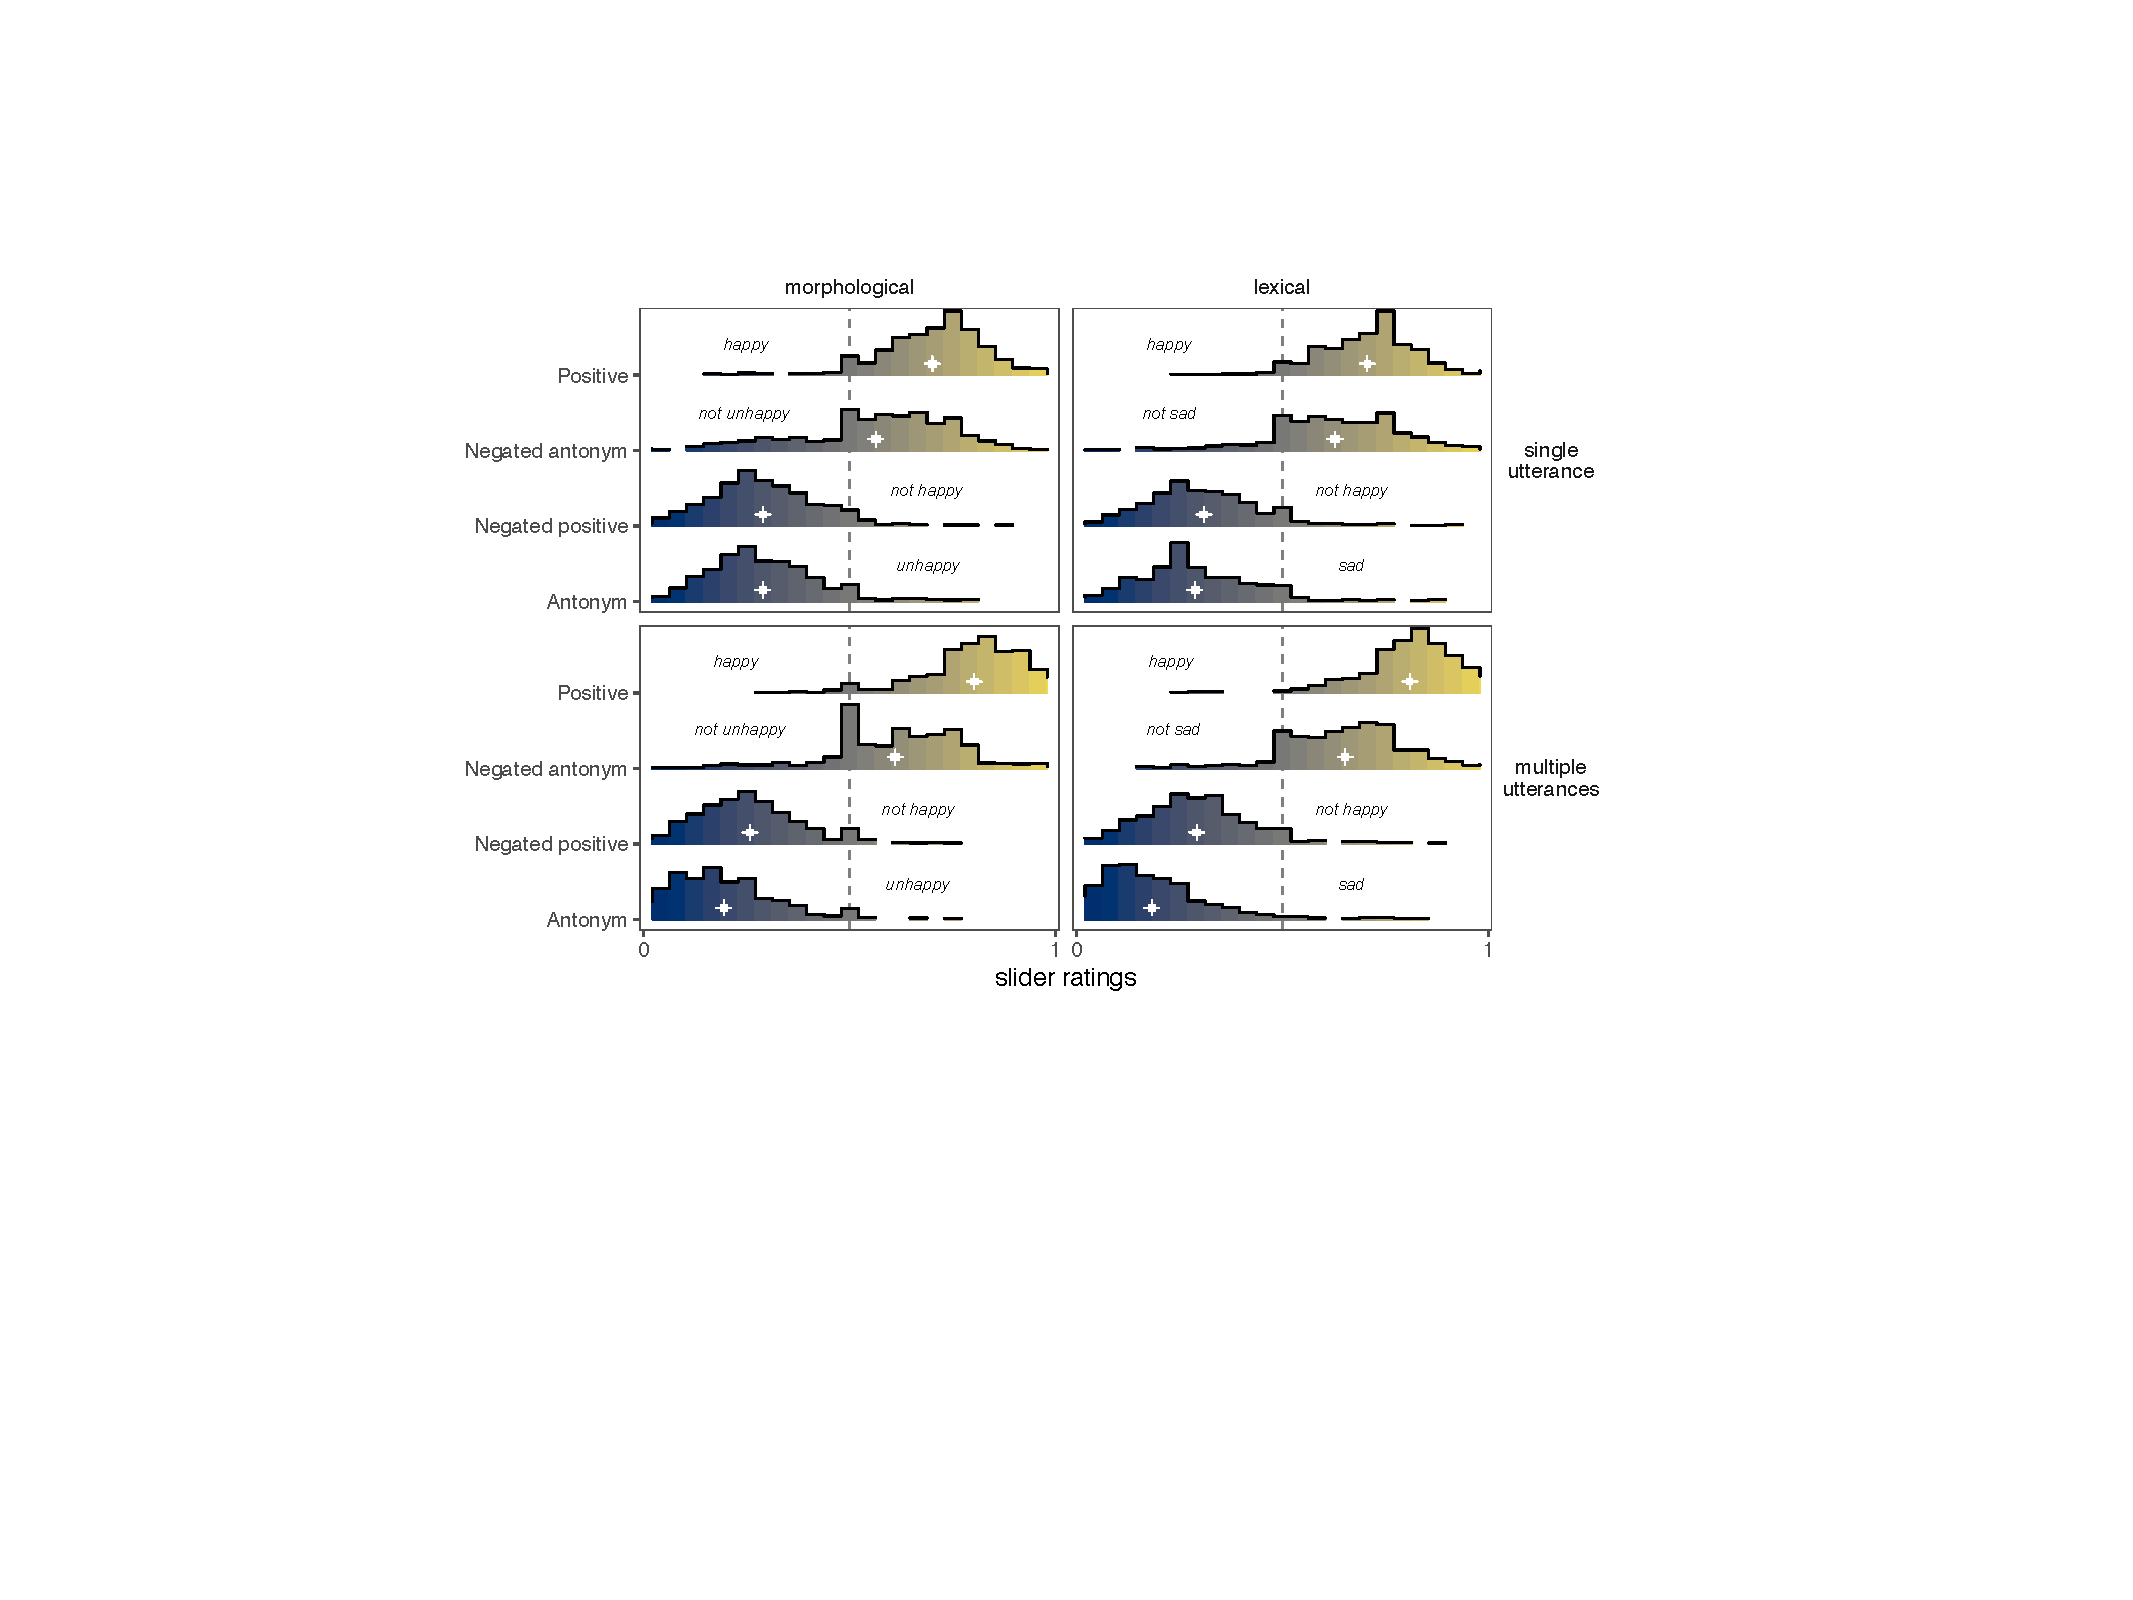
\includegraphics[width=0.95\linewidth]{figs/expt2_directlabel_hist} 
\caption{Experiment 2 results. Empirical histograms of responses for adjective sets with morphological antonyms (e.g., \emph{happy/unhappy}) and lexical antonyms (e.g., \emph{happy/sad}) for the single utterance and multiple utterances conditions. Dashed line indicates the midpoint of the scale. Width of white rectangles denotes bootstrapped 95\% confidence intervals for the means.}
\label{fig:expt2-results}
\end{figure}

As shown in Figure \ref{fig:modelPredictions}, the Flexible Negation model predicts that morphological antonyms (e.g., \emph{unhappy}) when heard in isolation should not be distinguished from negated positives (e.g., \emph{not happy}). This lack of interpretative difference stands in contrast to (1) lexical antonyms, which we predict should behave according to the Aristotelean model and show an interpretative difference between antonyms and negated positives and (2) hearing the adjectives in the same context, which is predicted by all models to exaggerate differences between adjectives, and specifically result in an interpretative difference between morphological antonyms and negated positives.
To test this, we built a Bayesian generalized linear mixed-effects model predicting the raw ratings in terms of fixed effects of \emph{adjective type}, \emph{antonym type} (morphological vs.~lexical),  and \emph{presentational context} (single~vs.~multiple utterances), and their pairwise two-way and three-way interactions; the model included a maximal random-effects structure with random intercepts, slopes of \emph{adjective type} by-participant, and random intercepts, slopes of \emph{adjective type}, \emph{antonym type}, \emph{presentational context}, and their pairwise two-way and three-way interactions by-item.

%As we did in \text{Experiment$\thinspace$1}, we evaluated our hypothesis that, in the \emph{single utterance condition}, morphological antonyms behave like the \emph{\ourmodel} model (i.e., show a partial ordering) while lexical antonyms show a true ordering (like \emph{bonafide contraries}).
%We considered data only from the \emph{single utterances} conditions and built a linear mixed model predicting the ratings normalized by-participant in terms of \emph{antonym type} (morphological vs.\text{~}lexical; dummy-coded with morphological as the base case), \emph{adjective type} (forward-difference coded in order: antonym, negated positive, negated antonym, positive) and their interaction; the model also included random intercepts and random slopes of \emph{adjective type} by-participant and by-item.

We predict that when heard in isolation, morphological antonyms will not show an interpretative difference between  \emph{antonyms} and \text{~}\emph{negated positives} (consistent with the \ourmodel model) while lexical antonyms will (consistent with the Aristotelean model).
Consistent with this hypothesis, in the single utterance conditions, the \emph{antonym} vs.\text{~}\emph{negated positive} difference was greater for lexical antonyms than morphological antonyms (i.e., an adjective type by antonym type interaction; \brmresultsp{expt2_brm_helmert_contrasts_10k.csv}{single_int_lex_morph_ant_v_negpos}; \effsize{expt2_brm_effsize_10k.csv}{single_int_lex_morph_ant_v_negpos}). 
At the same time, the \emph{antonym} vs.\text{~}\emph{negated positive} difference for morphological antonyms (e.g., \emph{unhappy} vs. \emph{not happy}) was not different from zero (\brmresultsp{expt2_brm_helmert_contrasts_10k.csv}{morph_single_ant_v_negpos}; \effsize{expt2_brm_effsize_10k.csv}{morph_single_ant_v_negpos}), while the contrast for lexical antonyms (e.g., \emph{sad} vs. \emph{not happy}) was greater than zero (\brmresultsp{expt2_brm_helmert_contrasts_10k.csv}{lex_single_ant_v_negpos}; \effsize{expt2_brm_effsize_10k.csv}{lex_single_ant_v_negpos}).

Our second prediction is that morphological antonyms will be interpreted differently than negated positive adjectives when they are heard in the same context.
%Our second main hypothesis is that context (single vs.\text{~}multiple utterances) modulates the interpretive difference between morphological antonyms and negated positives.
Specifically, we predict that morphological antonyms will be interpreted more negatively than negated positives in a context with multiple adjectival utterances.
Consistent with this prediction, the interpretative difference between morphological antonyms and negated positives varied as a function of context (i.e., an adjective type by context interaction; \brmresultsp{expt2_brm_helmert_contrasts_10k.csv}{morph_int_multi_single_ant_v_negpos}; \effsize{expt2_brm_effsize_10k.csv}{morph_int_multi_single_ant_v_negpos}). 
Morphological antonyms were not interpreted differently than negated positives when they were heard in isolation (single utterance condition; reported above), but they were interpreted differently when they were heard in the same context (multiple utterance condition; \brmresultsp{expt2_brm_helmert_contrasts_10k.csv}{morph_multi_ant_v_negpos}; \effsize{expt2_brm_effsize_10k.csv}{morph_multi_ant_v_negpos}).

%the \emph{antonym} vs.\text{~}\emph{negated positive} difference was greater for lexical antonyms than morphological antonyms (i.e., an adjective type by antonym type interaction; \brmresultsp{expt2_brm_contrasts_10k.csv}{single_int_lex_morph_negpos_v_ant}). 



%To evaluate this hypothesis, we considered data only from the morphological antonyms conditions and built a linear mixed model predicting the raw ratings in terms of \emph{adjective type} (forward-difference coded, as above),
%\emph{context} (single vs.~multiple utterances; multiple as base case) and their interaction; the model also included random intercepts and random slopes of adjective type by-participant and by-item.
%The \emph{antonym}~vs.~\emph{negated positive} difference was significantly greater in the \emph{multiple utterances} condition than the \emph{single utterance} condition (i.e., an adjective type by context interaction; \(\beta = \rlgetnum{expt2_glmer_morphological.csv}{Rowname}{conditionimplicit:adj_type1}{Estimate}{3}\), SE = 
%\rlgetnum{expt2_glmer_morphological.csv}{Rowname}{conditionimplicit:adj_type1}{Std..Error}{3}, t\((\rlgetnum{expt2_glmer_morphological.csv}{Rowname}{conditionimplicit:adj_type1}{df}{0}) = \rlgetnum{expt2_glmer_morphological.csv}{Rowname}{conditionimplicit:adj_type1}{t.value}{2}, p < 0.001\)), such that antonyms were interpreted more negatively than negated positives in the multiple utterances condition (\(\beta = \rlgetnum{expt2_glmer_morphological.csv}{Rowname}{adj_type1}{Estimate}{3}\), SE = 
%\rlgetnum{expt2_glmer_morphological.csv}{Rowname}{adj_type1}{Std..Error}{3}, t\((\rlgetnum{expt2_glmer_morphological.csv}{Rowname}{adj_type1}{df}{0}) = \rlgetnum{expt2_glmer_morphological.csv}{Rowname}{adj_type1}{t.value}{2}, p < 0.001\)), but not in the single utterance condition (same contrast as previous paragraph).


%Running the same model with the antonym type coded with lexical antonyms as the default level reveals that the \emph{antonym}~vs.~\emph{negated positive} contrast was significantly different for the lexical antonyms (e.g., \emph{sad} vs. \emph{not happy}; \(\beta =  \rlgetnum{expt2_glmer_singleUtt_lexBase.csv}{Rowname}{adj_type1}{Estimate}{3}
%\), SE = 
%\rlgetnum{expt2_glmer_singleUtt_lexBase.csv}{Rowname}{adj_type1}{Std..Error}{3}, t\(( \rlgetnum{expt2_glmer_singleUtt_lexBase.csv}{Rowname}{adj_type1}{df}{0}) =  \rlgetnum{expt2_glmer_singleUtt_lexBase.csv}{Rowname}{adj_type1}{t.value}{2}, p =  \rlgetnum{expt2_glmer_singleUtt_lexBase.csv}{Rowname}{adj_type1}{Pr...t..}{3}\)).



%\(\beta =  \rlgetnum{expt2_glmer_singleUtt.csv}{Rowname}{antonym_typelexant:adj_type1}{Estimate}{3}
%\), SE = 
%\rlgetnum{expt2_glmer_singleUtt.csv}{Rowname}{antonym_typelexant:adj_type1}{Std..Error}{3}, t\(( \rlgetnum{expt2_glmer_singleUtt.csv}{Rowname}{antonym_typelexant:adj_type1}{df}{0}) =  \rlgetnum{expt2_glmer_singleUtt.csv}{Rowname}{antonym_typelexant:adj_type1}{t.value}{2}, p =  \rlgetnum{expt2_glmer_singleUtt.csv}{Rowname}{antonym_typelexant:adj_type1}{Pr...t..}{3}\)).
%Further, the \emph{antonym} vs.\text{~}\emph{negated positive} difference for morphological antonyms (e.g., \emph{unhappy} vs. \emph{not happy}) was not significantly different from zero (\(\beta =  \rlgetnum{expt2_glmer_singleUtt.csv}{Rowname}{adj_type1}{Estimate}{3}
%\), SE = 
%\rlgetnum{expt2_glmer_singleUtt.csv}{Rowname}{adj_type1}{Std..Error}{3}, t\(( \rlgetnum{expt2_glmer_singleUtt.csv}{Rowname}{adj_type1}{df}{0}) =  \rlgetnum{expt2_glmer_singleUtt.csv}{Rowname}{adj_type1}{t.value}{2}, p =  \rlgetnum{expt2_glmer_singleUtt.csv}{Rowname}{adj_type1}{Pr...t..}{3}\)).
%Running the same model with the antonym type coded with lexical antonyms as the default level reveals that the \emph{antonym}~vs.~\emph{negated positive} contrast was significantly different for the lexical antonyms (e.g., \emph{sad} vs. \emph{not happy}; \(\beta =  \rlgetnum{expt2_glmer_singleUtt_lexBase.csv}{Rowname}{adj_type1}{Estimate}{3}
%\), SE = 
%\rlgetnum{expt2_glmer_singleUtt_lexBase.csv}{Rowname}{adj_type1}{Std..Error}{3}, t\(( \rlgetnum{expt2_glmer_singleUtt_lexBase.csv}{Rowname}{adj_type1}{df}{0}) =  \rlgetnum{expt2_glmer_singleUtt_lexBase.csv}{Rowname}{adj_type1}{t.value}{2}, p =  \rlgetnum{expt2_glmer_singleUtt_lexBase.csv}{Rowname}{adj_type1}{Pr...t..}{3}\)).

%We then analyzed the simple effects.
%Morphological antonyms were not significantly different than negated positives (\(\beta = \rlgetnum{expt2_glmer_singleUtt_morphological.csv}{Rowname}{adj_type1}{Estimate}{2}\), t\((\rlgetnum{expt2_glmer_singleUtt_morphological.csv}{Rowname}{adj_type1}{df}{0}) = \rlgetnum{expt2_glmer_singleUtt_morphological.csv}{Rowname}{adj_type1}{t.value}{3}, p = \rlgetnum{expt2_glmer_singleUtt_morphological.csv}{Rowname}{adj_type1}{Pr...t..}{3}\)), while lexical antonyms were interpreted more negatively than negated positives (\(\beta = \rlgetnum{expt2_glmer_singleUtt_lexical.csv}{Rowname}{adj_type1}{Estimate}{3}\), t\((\rlgetnum{expt2_glmer_singleUtt_lexical.csv}{Rowname}{adj_type1}{df}{0}) = \rlgetnum{expt2_glmer_singleUtt_lexical.csv}{Rowname}{adj_type1}{t.value}{2}, p < 0.001 \)).\footnote{The random effect structure for the simple effects models mirrored the full model. The only difference was that in analyzing the lexical antonyms, the random by-item slope for adjective type needed to be dropped in order for the model to converge.} \mf{Do we need to motivate for the reader why we ran two models here, but not in Experiment 1? (What did we preregister?)}


%\rlgetnum{expt2_glmer_singleUtt_lexical.csv}{Rowname}{adj_type1}{Pr...t..}{2}

%The relevant *antonym* vs. *negated positive* by adjective type (lexical, morphological) by context three-way interaction was in the direction of lexical antonyms showing a larger *antonym* vs. *negated positive* difference in the explicit context, but it was not significant ($\beta = `r round(rs3.3way.coef["adj_type1:antonym_typelexant:conditionexplicit","Estimate"],3)`$,  t$(`r round(rs3.3way.coef["adj_type1:antonym_typelexant:conditionexplicit","df"], 0)`) = `r round(rs3.3way.coef["adj_type1:antonym_typelexant:conditionexplicit","t value"],2)`, p = `r format(rs3.3way.coef["adj_type1:antonym_typelexant:conditionexplicit","Pr(>|t|)"], digits = 2)`$).


%\))).

% \rlgetnum{expt2_glmer_morphological.csv}{Rowname}{conditionexplicit:adj_type1}{Pr...t..}{2}

The predictions of the \ourmodel model (aimed at explaining morphological antonyms) and the Aristotelean model (aimed at explaining lexical antonyms) are ambiguous about the relevant three-way interaction (\emph{antonym} vs.~\emph{negated positive} by lexical vs.~morphological adjective type by context).
On the one hand, for the \emph{antonym} vs.~\emph{negated positive} contrast, we predict an interpretative difference for morphological antonyms only when the alternatives are presented together, whereas the difference is expected to occur for lexical antonyms in both context conditions.
On the other hand, pragmatics operates in both models (\ourmodel and Aristotle) to further differentiate the likely meaning of all of the adjectives as a result of being presented in the same context (i.e., all adjectives get more specific interpretations).
Thus, it is not clear \emph{a priori} what the prediction should be for the existence of a three-way interaction nor the direction of the interaction.
As an exploratory analysis, we examined the three-way interaction in our the regression model and found the relevant three-way interaction was in the direction of lexical antonyms showing a larger \emph{antonym} vs.~\emph{negated positive} difference in the multiple utterance condition (\brmresultsp{expt2_brm_helmert_contrasts_10k.csv}{int_multi_single_v_lex_morph_v_ant_negpos}; \effsize{expt2_brm_effsize_10k.csv}{int_multi_single_v_lex_morph_v_negpos_ant}). %, though (\(\beta =  \rlgetnum{expt2_glmer_full3way.csv}{Rowname}{adj_type1:antonym_typelexant:conditionexplicit}{Estimate}{3}
%\), SE = 
%\rlgetnum{expt2_glmer_full3way.csv}{Rowname}{adj_type1:antonym_typelexant:conditionexplicit}{Std..Error}{3}, t\(( \rlgetnum{expt2_glmer_full3way.csv}{Rowname}{adj_type1:antonym_typelexant:conditionexplicit}{df}{0}) =  \rlgetnum{expt2_glmer_full3way.csv}{Rowname}{adj_type1:antonym_typelexant:conditionexplicit}{t.value}{2}, p =  \rlgetnum{expt2_glmer_full3way.csv}{Rowname}{adj_type1:antonym_typelexant:conditionexplicit}{Pr...t..}{3}\)).
%\mf{maybe this paragraph could, if absolutely necessary, be dropped to save space?}

\section{Experiment 3: Flagrant Double Negatives}\label{experiment-3-notnot}

%We propose that the logic of negated morphological antonyms (\emph{not unhappy}) proceeds via a listener reasoning about why a speaker used two distinct negation markers (\emph{not} \& \emph{un-}) and concluding that the speaker must have had different meanings in mind (contradiction and contrary, respectively) for the different negation markers.
%Yet, the production of a double negative doesn't require distinct negation markers: One can grammatically produce a double negative flagrantly using the same negation marker twice (e.g., \emph{not not happy}).\footnote{While the usage of the same negation marker twice (e.g., \emph{not not}) is not common, examples are easy to find on webpages and news articles, suggesting that speakers use this construction to achieve real communicative goals.}

Is the inferential cognitive mechanism that produces meanings for negated antonyms specific to the usage of distinct negation markers (e.g., \emph{not} + \emph{un-}) or is it a more general mechanism that is triggered when two negatives are encountered?
%sufficiently flexible to accommodate double negations that rely upon the iterative application of the same logical word (\emph{not not})?
We investigate this question using flagrant double negatives like \emph{not not happy} in the \emph{multiple utterances} context from Experiment 2, with two different sets of alternative utterances. 
%Such a finding would suggest that communicative reasoning can contort one of the basic logical structures in language.
%The inference about the meaning of negation markers could be a general property of a speaker (i.e., this is how this speaker uses these negation markers) or may be a more specific inference about the particular usage of negation in context (i.e., in this moment, this is how this speaker intends to be understood when using negation). 
%If the inference is a specific inference about the particular usage of a negation marker, then the deployment of the same negation marker twice (e.g., \emph{not not happy}) should result in a meaning similar to that of negated morphological antonyms (e.g., \emph{not unhappy}). 
%Alternatively, if the inference occurs at the level of a particular speaker, the expression could only be a double contradiction and thus result in a meaning similar to that \emph{happy}. 
%In this experiment, we investigate interpretations of double ``not'' constructions using the \emph{multiple utterances} context from Experiment 2.

%Because we consider the status of negation markers to be \emph{a priori} uncertain, we use the \emph{multiple utterances} context from Experiment 2 to disambiguate the meaning of \emph{not} as conveying contradictory negation. 

\subsection{Experiment 3a: ``not not''}

In this experiment, we investigate the interpretation of a flagrantly double negative (e.g., \emph{not not happy}) when it appears in the same context as the other utterances from Expt.~2b: the positive adjective (e.g., \emph{happy}) and two negatives (e.g., \emph{not happy}, \emph{unhappy}).

\subsubsection{Methods}

\paragraph{Participants}\label{participants-3}

We recruited 75 participants from MTurk to match the sample size of the same condition in Expt.~2.
These numbers follow from the intention of getting approximately 45 ratings for each unique adjective in the experiment.
The experiment took on average 5 minutes and participants were compensated \$0.90.
Exclusion criterion, sample size, procedure, and the analysis described below were preregistered: \url{osf.io/vjhak}.

\paragraph{Materials and procedure}\label{materials-3}

The materials and procedure were identical to that of the \emph{multiple utterances} condition of Experiment~2.
The main difference in this experiment is that participants are presented with the following alternatives: positives, negated positives, morphological antonyms, and negated negated positives (e.g., \emph{happy}, \emph{not happy}, \emph{unhappy}, \emph{not not happy}).
This experiment was conducted eighteen months after Experiment~2, and due to concerns about recently declining data quality on MTurk, this experiment included an additional memory check wherein participants had to select all of the items that they recall being tested on from a list of 10 items (5 real and 5 distractor). 
We pre-registered the exclusion criterion of removing participants who failed to respond correctly to at least 7 of the 10 items. 


\subsubsection{Results}

All participants self-reported only English as their native language. Five participants were excluded for failing to respond correctly to at least 7 of the 10 memory check items, leaving 40 participants for these analyses.
Figure \ref{fig:expt3-results} shows results for each adjective type.

Our main hypothesis concerns the interpretation of flagrant double negative statements that use the same negation marker twice (\emph{not not happy}). 
We built a Bayesian mixed-effects regression model with random by-participant and by-item intercepts and slopes (where the slopes refer to the effect of the adjective type, forward-difference coded as before: happy vs.~not happy vs.~not not happy vs.~unhappy).
The two negatives did not simply cancel to make a positive: \emph{not not happy} received a substantially more negative interpretation than \emph{happy} (\brmresultsp{expt3_brm_contrasts_10k.csv}{morph_negnegpos_v_pos}; \effsize{expt3_brm_effsize_10k.csv}{morph_negnegpos_v_pos}).
This results suggests that participants actively try to make sense of seemingly redundant, contradictory information in a way that would be informative for a speaker to produce. 
In addition, we replicate the result from Experiment 2 (multiple utterances condition) for the morphological antonyms vs. negated positives difference: \emph{not happy} and \emph{unhappy} were differentiated in meaning (\brmresultsp{expt3_brm_contrasts_10k.csv}{morph_ant_v_negpos}; \effsize{expt3_brm_effsize_10k.csv}{morph_ant_v_negpos}).
Contrary to our hypothesis, however, we did not find evidence that the flagrant double negative \emph{not not happy} received on-average a positive interpretation \brmresults{expt3_brm_contrasts_10k.csv}{negnegpos}; inspection of the fitted random-effects suggested this was due to large subject-wise variation in the interpretation of these flagrant double negatives. 
We return to this observation in the General Discussion. 

%\mht{should we discuss the felicity of ``not not''? a google search reveals that people are using it...} 

%\mf{I don't think that we have to}

\subsection{Experiment 3b: ``not not''~vs.~``not un-''}

In Expt.~3b, we directly compare the interpretation of two double negatives when observed in the same context (e.g., \emph{not not happy}~vs.~\emph{not unhappy}).

\subsubsection{Methods}

\paragraph{Participants}\label{participants-3}

We recruited 50 participants from MTurk. 
This number was arrived at with the intention of getting approximately 20 ratings for each unique item in the experiment.
The experiment took on average 5 minutes and participants were compensated \$1.00.
Exclusion criterion, sample size, procedure, and the analysis described below were preregistered: \url{https://osf.io/5zqd7}.

\paragraph{Materials and procedure}\label{materials-3}

The materials and procedure were almost identical to that of the \emph{multiple utterances} condition of Experiment~2 and Experiment 3a.
In this experiment, participants were presented with five  alternatives: positive adjectives, negated positives, morphological antonyms, negated morphological antonyms, and negated negated positives (e.g., \emph{happy}, \emph{not happy}, \emph{unhappy}, \emph{not unhappy}, \emph{not not happy}).
Since we observed substantially greater participant-wise variability than item-wise variability in Expt.~3a, we decided to shorten the experiment so participants completed 8 trials instead of the 12 used in Experiment 3a.
As with Experiment 3a, this experiment included an additional memory check wherein participants had to select all of the items that they recall being tested on from a list of 10 items (5 real and 5 distractor). 
We pre-registered the exclusion criterion of removing participants who failed to respond correctly to at least 7 of the 10 items. 

\begin{figure}[h]
\centering 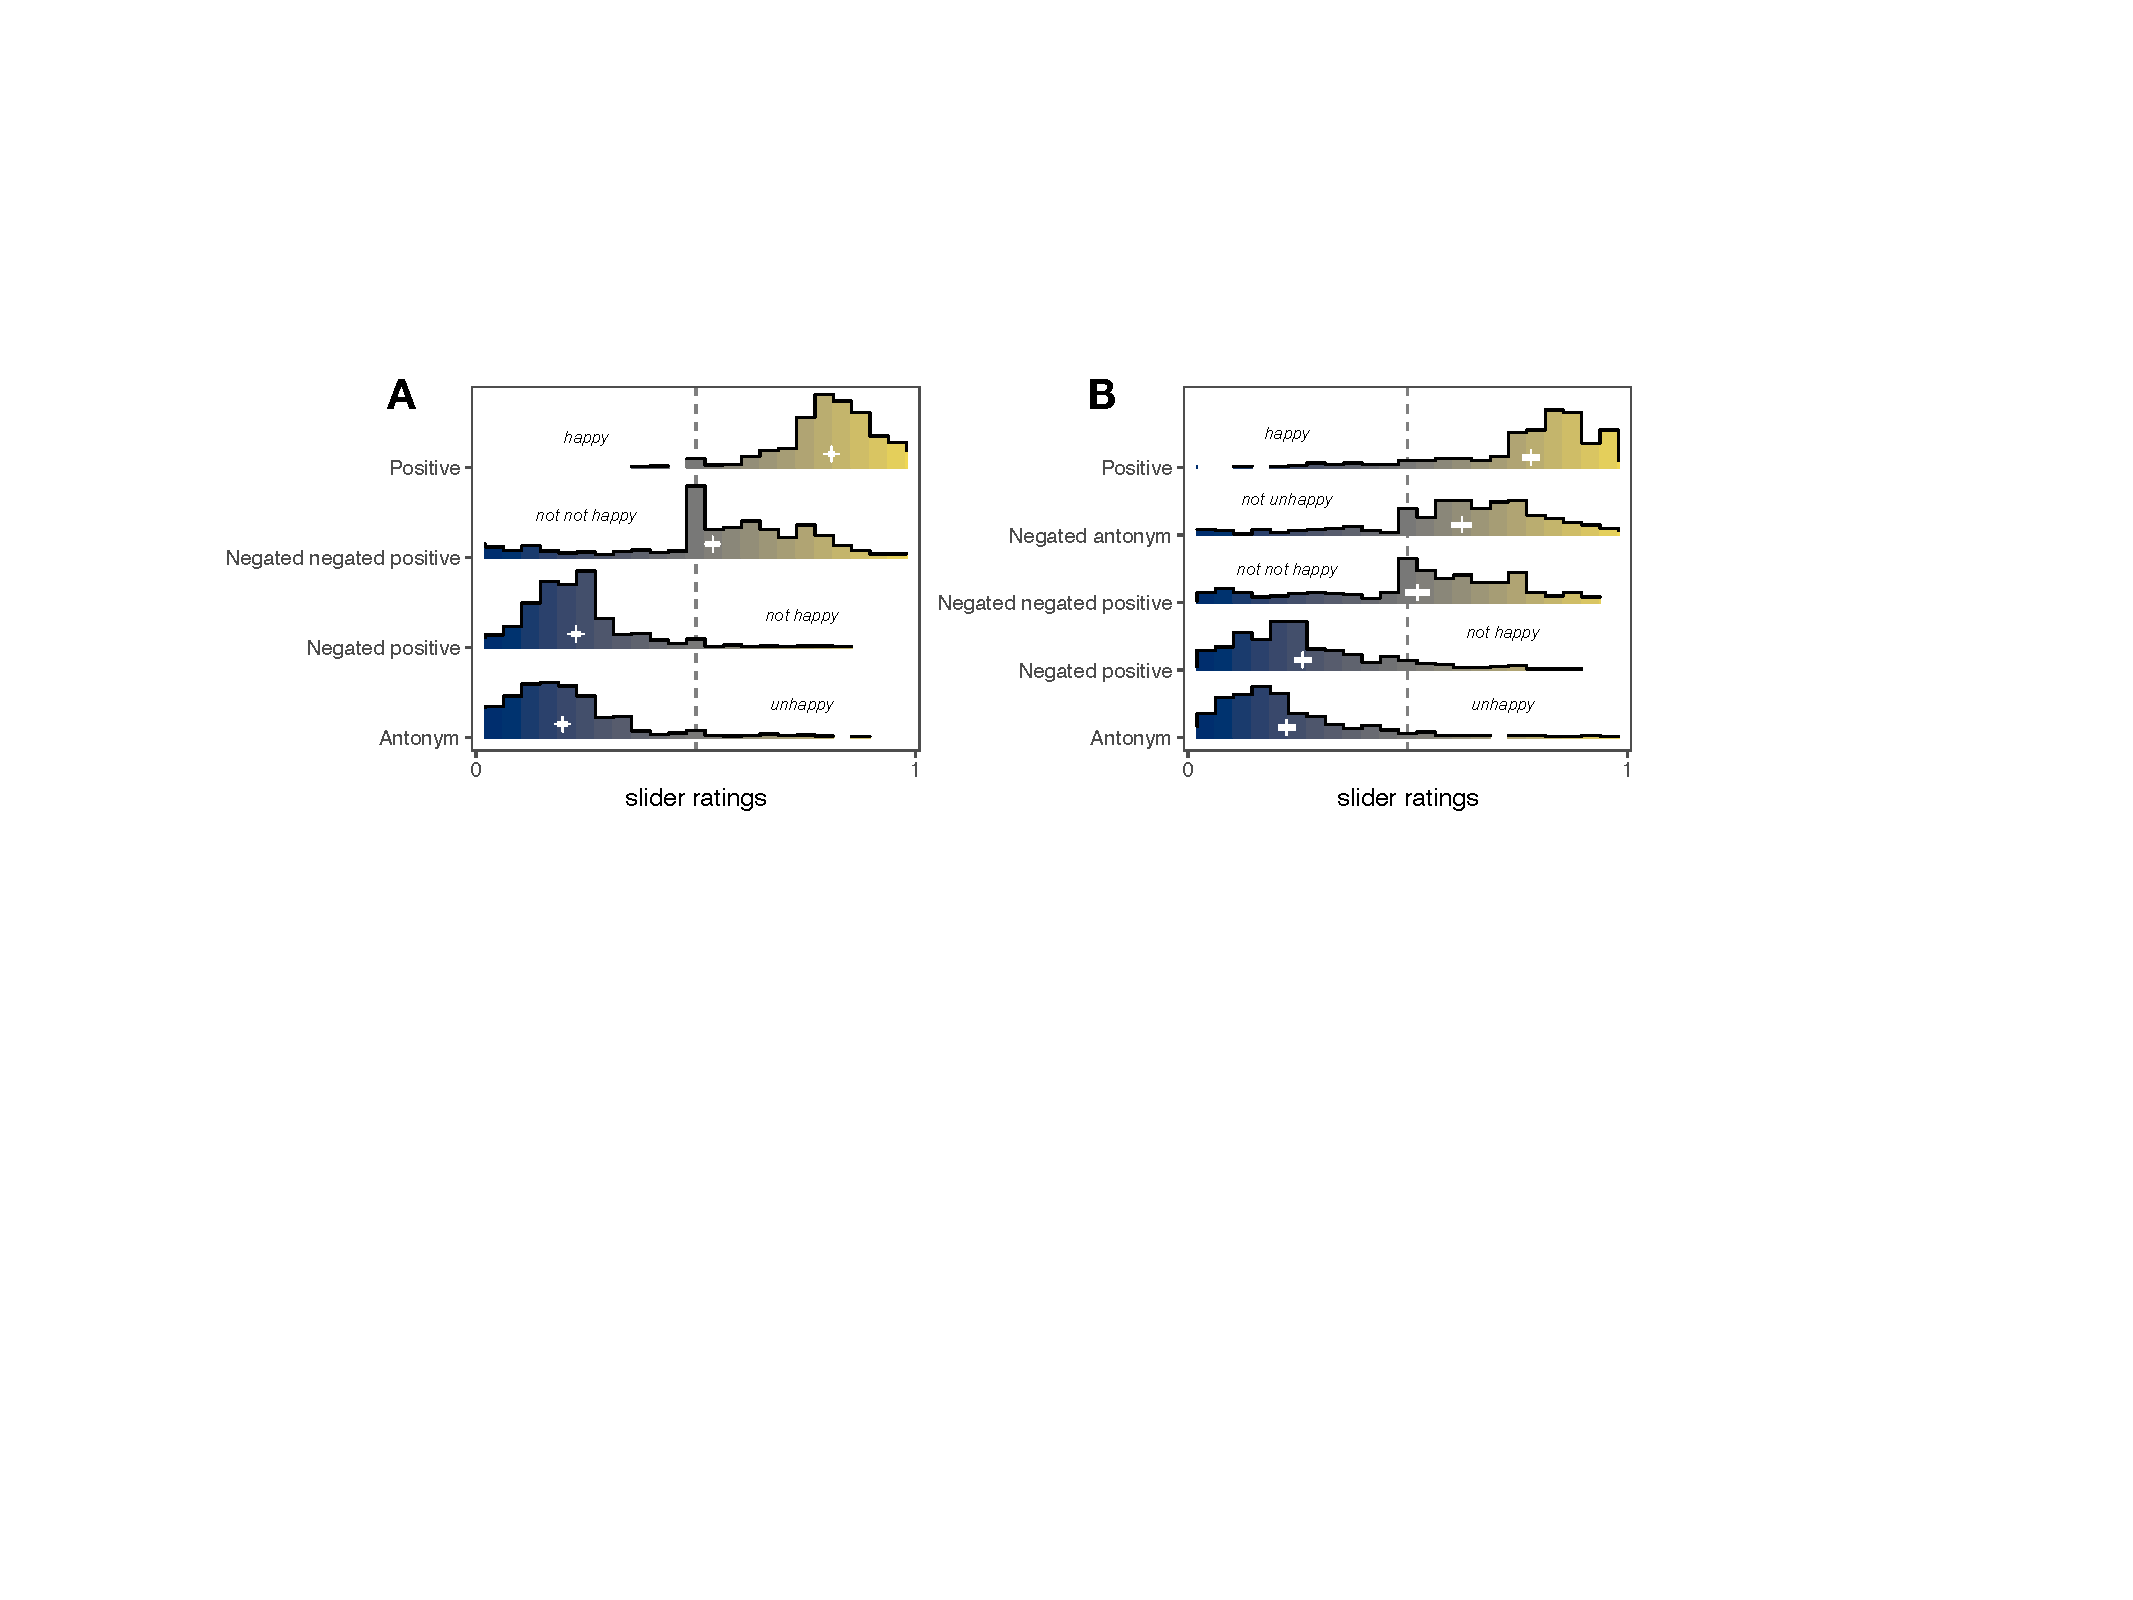
\includegraphics[width=\linewidth]{figs/expt3_directlabel_hist_ab} 
\caption{Experiment 3 results. A: Experiment 3a in which the doubly-negated adjective is presented in the context of the positive adjective, the morphological antonym, and the negated adjective. B: Experiment 3b in which the doubly-negated adjective is presented in the context of the same alternatives and the negated morphological antonym. Dashed line indicates scale midpoint. White bars denote bootstrapped 95\% confidence intervals for the means.}\label{fig:expt3-results}
\end{figure}


\subsubsection{Results}

1 participant self-reported a language other than English as their native language. 
An additional 12 participants were excluded for failing to respond correctly to at least 7 of the 10 memory check items, leaving 37 participants for these analyses.
Figure \ref{fig:expt3-results}b shows results for each adjective type.

In this experiment, we are concerned with whether or not participants will draw an interpretative difference between negated morphological antonyms (e.g., \emph{not unhappy}) and doubly negated positives (e.g., \emph{not not happy}).
We built a Bayesian mixed-effects regression model with random by-participant and by-item intercepts and slopes (where the slopes refer to the effect of the adjective type).
As suggested by Experiment 3a in which the two double negatives are not presented in the same context, the doubly-negated positive adjective receives a lower overall rating than the negated morphological antonym (\brmresultsp{expt3b_brm_contrasts_10k.csv}{morph_negnegpos_v_negant}; \effsize{expt3b_brm_effsize_10k.csv}{morph_negnegpos_v_negant}).
As in Experiment 3a, doubly-negated positive adjectives receive on average a rating not distinguished from the midpoint (\brmresultsp{expt3b_brm_contrasts_10k.csv}{negnegpos}; \effsize{expt3b_brm_effsize_10k.csv}{negnegpos}).

Examining the distribution of responses for \emph{not not happy} vs. \emph{not unhappy}, we observe that the negated negated adjective (\emph{not not happy}) receives about twice as many negative responses (i.e., responses lower than the mid-point of the scale, assuming a 5-pt buffer on the 101-pt scale, or responses $< 0.45$ on the scale; 27\%~vs.~14\%) and about twice as many mid-point responses (assuming a 5-pt buffer; $0.45 <$ response $< 0.55$; 20\%~vs~11\%) than the negated morphological antonym (\emph{not unhappy}). This variability in responses suggests that listeners will try to rationalize a speaker who flagrantly contradicting themselves, and can use a variety of strategies to do so.

Finally, we replicate the previous results from Experiment 2 (multiple utterances condition) and Experiment 3a in which \emph{not happy} and \emph{unhappy} are subtly differentiated in meaning (\brmresultsp{expt3b_brm_contrasts_10k.csv}{morph_ant_v_negpos}; \effsize{expt3b_brm_effsize_10k.csv}{morph_ant_v_negpos}).



%\hypertarget{discussion}{%
\section{General Discussion}\label{discussion}

%\mht{Discuss Horn's analysis as division of pragmatic labor. Does the fact that we need some cost for this to get off the ground provide some resonance for Horn (1991)'s analysis?}
%}
%\mht{this opening paragraph is more about vagueness than \ourmodel...}
%Many dimensions that language can pick out have no units.
%Speakers cannot say they are \emph{42 units happy} like they can say they are \emph{6'1" tall}.
%Instead, speakers can use modifiers and morphemes to carve more precise meanings from otherwise vague dimensions.
%A person \emph{not unhappy} is neither sad nor truly happy, but residing in some marginally positive state that is difficult to refer to because degrees of happiness lack precise units.

Understanding language is a holistic process in which many factors---the meanings of words, uncertainty, the communicative process---come together to produce interpretations. Pragmatics (or, communicative reasoning), in particular, is a complicated, elusive, and often-ignored factor that is necessary to consider to understand how the meanings of words are computed in context. 
Across three experiments using a straight-forward response measure, we find the interpretations of natural language negation can change based on the subtle contextual circumstance of the presence of other uses of negation in the same context.
These findings highlight just how deep the flexibility and context-sensitivity of language run, and underscore the importance of discarding simplistic pictures of language understanding that assume transparent and static meanings of the words used in a sentence. 

%From the study of logical language in both experiments of human reasoning and naturalistic uses in legal contexts to any study that uses language to convey the instructions or experimental manipulations of a study, we must do away with simple pictures of language that would assume transparent and static meanings of the words used in a sentence. 


We provide a computational solution to an outstanding puzzle in natural language understanding: How to interpret double negatives \cite<e.g., \emph{not unhappy}; >{Horn1991:Duplex, Krifka2007:Negated-antonyms, Rett2014:eval}.
We additionally discovered and confirmed a surprising empirical result: \emph{unhappy} (morphological antonyms) and \emph{not happy} (negated positives) are interpreted identically, except when heard in the same context.
Our model that represents flexibility in how to interpret negation markers (\emph{un-}, \emph{not}) predicts this very result, while alternative models that treat negation markers as only carrying a single possible meaning fall short.

We predicted and observed empirically the ordering hypothesized by \citeA{Krifka2007:Negated-antonyms} for morphological antonyms (\emph{unhappy} $<$ \emph{not happy} $<$ \emph{not unhappy} $<$ \emph{happy}), when a listener hears multiple adjectival utterances in the same context (Experiment 2; \emph{multiple utterances condition}).
Other accounts derive similar predictions based on different kinds of assumptions \cite{Krifka2007:Negated-antonyms, Rett2014:eval, Cable2017}, but only our model makes predictions about the context-dependence of these inferences.
This work thus carries with it an account of a robust linguistic intuition: Potentially equivalent utterances receive differential interpretations when produced by the same speaker in close proximity, an instance of \emph{mutual exclusivity} reasoning \cite{Markman1989}. %\mht{are the other lexical uncertainty papers not an instance of this general point as well?}
%\mf{I think so. But we do set ourselves off. Maybe like so: ""
%More generally, the inferences modeled here can be seen as an instance of \emph{mutual exclusivity} \cite{Markman1989}, in which listeners resolve uncertainty about multiple elements of meaning simultaneously.
%Reasoning about multiple meanings for words, listeners conclude that a choice of different expressions may be most likely for a speaker who differentiates meanings.
In Experiment 3, we discovered that this inference goes beyond using distinct  negation markers: Expressions that use the same negation marker twice (e.g., \emph{not not happy}) are interpreted similarly to negated morphological antonyms (e.g., \emph{not unhappy}). 
This result points to an underlying cognitive mechanism that flexibly allows for different meanings for the same negation marker within a single utterance, guided by a principled logic: A contradiction of a contrary is a pragmatically useful double negative. 

We build upon previous studies on negated adjectives \cite<e.g., >{giora2005negation} with our straight-forward response measurements, comparison of morphological and lexical antonyms, and situation within different presentational contexts.
%We extend earlier work showing that negated lexical antonyms (e.g., \emph{not dull}) are distinct from positive adjectives (e.g., \emph{sharp}) when presented simultaneously \cite{giora2005negation} to both the case of morphological antonyms (e.g., \emph{not unhappy}) and when presented in isolation (single utterance conditions). 
%ound that participants rate . 
We also provide convergent evidence that supports the phenomenon of \emph{negative strengthening} or \emph{inference towards the antonym}, where negating an adjective (e.g., \emph{not intelligent}) can lead to the stronger interpretation than literally implied \cite<e.g.,  rather stupid;>{Ruytenbeek2017, Gotzner2018}. 
%Not only do 
%Our empirical data further elucidate these phenomena with our straight-forward response measurements and comparisons to other adjective forms in different presentational contexts.%, our modeling approach provides an explanation for negative strengthening through uncertainty about the meaning of negation markers (i.e., \emph{not} could signal a contrary meaning). 
%\mf{I feel iffy about the last sentence, and would even like to drop it. My understanding is that the reason why we predict a slightly positive interpretation of \emph{not short}, has nothing to do with flexibly uncertain negation. We predict it also for set-ups with only \emph{not} and no uncertainty at all, right? It's also dubious that what we predict is \emph{negative strengthening} which is bound to the negatively-connotated form. We predict the reversed pattern ``positive strengthening'' as well. But that actually shows that (i) we do not predict what the linguists call negative strengthening, and (ii) what looks like it is not predicted by the mechanism mentioned above.}


%\mf{These last two sentences (and the whole framing and discussion of Exp 3 are problematic. My understanding of our account of the difference between \emph{unhappy} and \emph{happy} is that it hinges on observing the same speaker use \emph{not unhappy}, which is only rational for speakers with a \emph{\textbf{fixed (!!!)}} lexicon of allocations of negation markers to meanings. If we allow individual occurrences of negation markers to be interpreted individually, that explanation would break. --- It may be possible to explain the \emph{not not happy} case as a last resort: normally, we would assume that speakers use negation markers consistently, \emph{unless that assumption would blatantly violate rationality}, i.e., trying to express a meaning for which there is an equivalent but less costly form. But even in that case we have a problem: how do we account for the divergence of \emph{unhappy} and \emph{not happy} in the case where \emph{not unhappy} is not present, but \emph{not not happy} is?}

%In our final experiment, we showed that receive an interpretation similar to that of more conventional 

%The fact that \emph{not not happy} is differentiated in meaning from the simple \emph{happy} suggests the same word (\emph{not}) can be interpreted in two different ways within a single utterance  (i.e., conveying both contradictory and contrary negation). 
% where the uncertainty 
%%At the same time, expressions of double negation (\emph{not not}, \emph{not un-}) were not differentiated by listeners even when presented in the same context, suggesting that language understanding respects the logical possibilities that the rules of semantic opposition permit  \cite{Horn1989:Natural}.
%These results suggest both a radical but bounded view of the uncertainty of linguistic expressions. 

Our formalization of lexical uncertainty about the meaning of natural language negation adds to a growing movement to treat the combinatorial rules of grammar as not entirely separable from the lexicon \cite<e.g., >{bybee2006usage, Odonnell2015productivity}.
Psycholinguistic evidence supports the idea that commonly used utterances are processed as unique lexical entries while less frequent phrases are interpreted compositionally \cite{MorganLevy2016:binomials}.
The two types of negation meaning we considered---contrary and contradictory opposition---can be seen as a \emph{lexicalized} form of opposition and a \emph{compositional} rule, respectively.\footnote{
Contraries act as a lexicalized form of negation because their meanings refer to semantic variables distinct from the positive adjective (in particular, a different threshold; see SI), whereas contradictions refer to the same semantic variable as the positive adjective. 
}
In our modeling, we assumed all logically possible meanings for negation were equally likely \emph{a priori}: A further test of our negation uncertainty model would be to see if usage frequency can serve as a proxy for this prior over lexica.

Our model explains the modal interpretations of antonym pairs and their negations, but our empirical data suggest more nuance and variability in judgments, even in our minimal paradigms.
While the modal response for negated antonyms was indicating a slightly positive state, there were consistent  responses indicating a slightly negative interpretation as well (e.g., the meaning expressed by ``he's not [un]reliable \emph{but he is kind of flaky}'', with prosodic focus on [un-]), potentially the result of politeness \cite{Yoon2017}.
%This interpretation may be the result of participants attributing politeness to the speaker: \emph{Not unreliable} may be an indirect way of saying that a person is not reliable \cite{Yoon2017}.
We also see a hint of strongly negative interpretations (e.g., very unhappy) from the flagrant double negatives of Experiment 3 (\emph{not not happy}): The additivity of negations, or \emph{negative concord}, is not often associated with standard English, though it is relatively common cross-linguistically \cite<e.g., in Italian: \emph{non capisco niente}, literal translation: \emph{I don't understand nothing; }>{zeijlstra2004sentential} including in African American Vernacular English \cite<e.g., Mohammad Ali: ``Ain't never been another fighter like me''; >{labov1972negative, howe2005negation}.
%Finally, though we did not find evidence of double negatives being interpreted as strong positives in our minimal experimental contexts, double negatives  are employed in understatement \cite{bolinger1972degree}: In the appropriate context, ``I was not unaware of the problem'' could mean \emph{I was damn well aware}.
%\red{[Horn ``not unaware'']}
%\red{[midpoint responses? ]}
%All our experiments involve utterances conveyed in text with minimal contexts;
Future work should investigate the relevant context and prosodic cues that can be used to derive diverse interpretations from antonym pairs and their negations.
Additionally, though our experiments are conducted in English, we expect these patterns to hold cross-linguistically for languages without negative concord and with the negation markers that can act as productively as English \emph{not} and \emph{un-}. 


The meaning of explicit negation markers like \emph{not} and \emph{un-} is flexible, allowing for an ambiguity that can be exploited by speakers.
Our results suggest that if a speaker claims an individual is \emph{not not innocent}, the speaker could simultaneously convey that the person is innocent as well as at least somewhat guilty.
Such obfuscation can lead to confusion within listeners or divergent beliefs across listeners, with some people believing in innocence and others in guilt as a kind of ``dog whistle''.
It may as well impose gradability (e.g., degrees of guilt) onto what would typically be a binary distinction (i.e., innocent or guilty). 
Understanding the psychological reality of this ambiguity will help us navigate the consequences of the plausibly deniable misinformation that lays in the language of negation.


%To negate is to make true false, but for statements that are truly vague, the behavior of negation is not so obvious.
%We present a computational explanation for why this is so, and provide empirical data that sheds new light on the age old question of meaning and opposition.

%\mht{other thoughts: (a) dimensionality in antonyms (unhappy and sad map onto slightly different dimensions); (b) how much of this is specific to (American) English? [there is an oft intuition that Orwell believes this because he is british]; (c) relation to understatement more broadly}


%This result suggests a radical uncertainty model, where the meanings of linguistic expressions are computed on the fly
%Our final experiment challenges rigid views of language 
%One limitation of this work is that we stipulate, rather than derive, differences in meaning for morphological vs.~lexical antonym pairs (cf., Rett, 2014).


\newpage

%\hypertarget{references}{%
%\section{References}\label{references}%}

\bibliographystyle{apacite}

\setlength{\bibleftmargin}{.125in}
\setlength{\bibindent}{-\bibleftmargin}

\bibliography{negant}
%
%\begingroup
%\setlength{\parindent}{-0.5in}
%\setlength{\leftskip}{0.5in}
%
%\hypertarget{refs}{}
%\leavevmode\hypertarget{ref-lme4}{}%
%Bates, D., M\wrapmf{\"{a}}chler, M., Bolker, B., \& Walker, S. (2015). Fitting linear mixed-effects models using lme4. \emph{Journal of Statistical Software}, \emph{67}(1), 1--48.
%
%\leavevmode\hypertarget{ref-Bergen2016}{}%
%Bergen, L., Levy, R., \& Goodman, N. D. (2016). Pragmatic reasoning through semantic inference. \emph{Semantics and Pragmatics}, \emph{9}.
%
%\leavevmode\hypertarget{ref-Blutner2004:pragmatics}{}%
%Blutner, R. (2004). Pragmatics and the lexicon. \emph{Handbook of Pragmatics}, \emph{488514}.
%
%\leavevmode\hypertarget{ref-bybee2006usage}{}%
%Bybee, J. L. (2006). From usage to grammar: The mind's response to repetition. \emph{Language}, \emph{82}(4), 711--733.
%
%\leavevmode\hypertarget{ref-Cable2017}{}%
%Cable, S. (2017). The good, the 'not good', and the 'not pretty': Negation in the negative predicates of tlingit.
%
%\leavevmode\hypertarget{ref-Franke2015a}{}%
%Franke, M., \& J\wrapmf{\"{a}}ger, G. (2015). Probabilistic pragmatics, or why Bayes' rule is probably important for pragmatics. In \emph{Zeitschrift für sprachwissenschaft} (pp. 3--44).
%
%\leavevmode\hypertarget{ref-Goodman2016:RSA}{}%
%Goodman, N. D., \& Frank, M. C. (2016). Pragmatic language interpretation as probabilistic inference. \emph{Trends in Cognitive Sciences}, \emph{20}(11), 818--829.
%
%\leavevmode\hypertarget{ref-Horn1989:Natural}{}%
%Horn, L. R. (1989). \emph{A natural history of negation}. University of Chicago Press.
%
%\leavevmode\hypertarget{ref-Horn1991:Duplex}{}%
%Horn, L. R. (1991). Duplex negatio affirmat...: the economy of double negation. \emph{CLS 27-II: Papers from the Parasession on Negation}, 80--106.
%
%\leavevmode\hypertarget{ref-Jespersen1917:Negation}{}%
%Jespersen, O. (1917). \emph{Negation in english and other languages}. Kobenhavn: Host.
%
%\leavevmode\hypertarget{ref-Jespersen1924}{}%
%Jespersen, O. (1924). \emph{The philosophy of grammar}. London: Allen \& Unwin.
%
%\leavevmode\hypertarget{ref-Kennedy2007}{}%
%Kennedy, C. (2007). Vagueness and grammar: the semantics of relative and absolute gradable adjectives. \emph{Linguistics and Philosophy}, \emph{30}, 1--35.
%
%\leavevmode\hypertarget{ref-Krifka2007:Negated-antonyms}{}%
%Krifka, M. (2007). Negated Antonyms: Creating and Filling the Gap. \emph{Presupposition and Implicature in Compositional Semantics}, 163--177.
%
%\leavevmode\hypertarget{ref-Lassiter2015}{}%
%Lassiter, D., \& Goodman, N. D. (2015). Adjectival vagueness in a Bayesian model of interpretation. \emph{Synthese}.
%
%\leavevmode\hypertarget{ref-Markman1989}{}%
%Markman, E. M. (1989). \emph{Categorization and naming in children: Problems of induction}. MIT Press.
%
%\leavevmode\hypertarget{ref-MorganLevy2016:binomials}{}%
%Morgan, E., \& Levy, R. (2016). Abstract knowledge versus direct experience in processing of binomial expressions. \emph{Cognition}, \emph{157}, 384--402.
%
%\leavevmode\hypertarget{ref-Odonnell2015productivity}{}%
%O'Donnell, T. J. (2015). \emph{Productivity and reuse in language: A theory of linguistic computation and storage}. MIT Press.
%
%\leavevmode\hypertarget{ref-Rett2014:eval}{}%
%Rett, J. (2014). \emph{The semantics of evaluativity}. Oxford University Press.
%
%\leavevmode\hypertarget{ref-Yoon2017}{}%
%Yoon, E. J., Tessler, M. H., Goodman, N. D., \& Frank, M. C. (2017). "I won't lie, it wasn't amazing": Modeling polite indirect speech. In \emph{Proceedings of the 39th annual meeting of the cognitive science society}.
%
%\endgroup


\end{document}

;; Local Variables:
;; eval: (auto-fill-mode -1)
;; End:
